\documentclass{article}
% The original PRIMEarxiv format is used if its style file is present.
% This complete main.tex also compiles directly in a new Overleaf project
% without additional downloads using a compatible article fallback.
\IfFileExists{PRIMEarxiv.sty}{\usepackage{PRIMEarxiv}}{\usepackage[letterpaper,margin=0.90in,headheight=14pt]{geometry}\usepackage{lmodern}}
\IfFileExists{PRIMEarxiv.sty}{\newcommand{\PaperAuthorSep}{\And}}{\newcommand{\PaperAuthorSep}{\and}}
\providecommand{\keywords}[1]{\par\medskip\noindent\textbf{Keywords:} \begingroup\def\and{\unskip\space$\cdot$\space}#1\endgroup\par}
\usepackage[utf8]{inputenc}
\usepackage[T1]{fontenc}
\usepackage{microtype}
\usepackage{amsmath,amssymb,amsfonts,amsthm,mathtools}
\usepackage{booktabs,tabularx,multirow,array}
\usepackage{graphicx}
\usepackage[dvipsnames]{xcolor}
\usepackage{tikz}
\usetikzlibrary{arrows.meta,positioning,patterns,calc,fit,backgrounds,shapes.geometric}
\usepackage[unicode,hidelinks]{hyperref}
\usepackage{url,xurl,seqsplit}
\hypersetup{
  pdftitle={Executable Source Contracts for Architecture-Aware FPGA Neural-Network Compilation},
  pdfauthor={Umut Can Altin; Marcel van Gerven},
  pdfsubject={Architecture-aware FPGA neural-network compilation and contract-aware source semantics}
}
\usepackage{fancyhdr}
\usepackage{enumitem}
\usepackage{caption}
\captionsetup[table]{font=small,labelfont=bf,justification=raggedright,singlelinecheck=false,skip=5pt}
\newcommand{\tablenote}[1]{\par\vspace{3pt}\begin{minipage}{\linewidth}\footnotesize\emph{Note.} #1\end{minipage}}
\usepackage{float}
\usepackage{cleveref}
\definecolor{navy}{HTML}{20354D}
\definecolor{darkteal}{HTML}{216B79}
\definecolor{muted}{HTML}{566473}
\definecolor{pale}{HTML}{F1F5F7}
\definecolor{warmgray}{HTML}{E8EBEF}
\definecolor{lightgray}{gray}{0.94}
\tikzset{
  every node/.append style={font=\sffamily\scriptsize},
  nohyph/.style={execute at begin node={\hyphenpenalty=10000\exhyphenpenalty=10000\relax}},
  box/.style={draw,rectangle,rounded corners=1.4pt,line width=0.6pt,inner xsep=4pt,inner ysep=3.5pt,align=center,fill=white,nohyph},
  sem/.style={box}, arch/.style={box,fill=black!8},
  phys/.style={box,double,double distance=0.8pt},
  stage/.style={box,line width=1.1pt},
  flow/.style={-{Latex[length=1.9mm,width=1.4mm]},line width=0.7pt},
  meta/.style={-{Latex[length=1.5mm,width=1.1mm]},line width=0.5pt,densely dashed,black!60},
  ttl/.style={font=\sffamily\footnotesize\bfseries},
  note/.style={font=\sffamily\scriptsize\itshape,text=black!70,align=center,nohyph},
  elab/.style={font=\sffamily\scriptsize\itshape,text=black!70,inner sep=0.8pt,align=center},
  contract/.style={box,fill=black!5},derived/.style={box,dashed},
  evidence/.style={box,dotted,line width=0.8pt},divider/.style={black!35,line width=0.5pt}
}
\newcommand{\ft}[1]{{\footnotesize\bfseries #1}}
\newcommand{\doilink}[1]{\href{https://doi.org/#1}{doi:#1}}
\newtheorem{proposition}{Proposition}
\newcommand{\cert}{\mathsf{certified}}
\newcommand{\reject}{\mathsf{rejected}}
\newcommand{\unknown}{\mathsf{uncertified}}
\newcommand{\src}{\mathsf{src}}
\newcommand{\HLS}{\mathsf{HLS}}
\newcommand{\obs}{\Omega}
\newcommand{\trans}{\mathcal{T}}
\newcommand{\mask}{\mathcal{M}}
\pagestyle{fancy}
\fancyhf{}
\fancyhead[L]{\footnotesize FPGAI: Contract-Aware Model IR and Source Verification}
\fancyhead[R]{\footnotesize\textit{Research preprint}}
\fancyfoot[C]{\thepage}
\renewcommand{\headrulewidth}{0.35pt}
\setlist[itemize]{nosep,leftmargin=1.3em}
\emergencystretch=2em
\title{Executable Source Contracts for Architecture-Aware FPGA Neural-Network Compilation}
% The two authors are presented in the same typeface, size, and weight.
% \normalfont explicitly overrides any bold default in PRIMEarxiv title styles.
\author{%
{\normalfont\large Umut Can Alt\i{}n} \\[2pt]
{\normalfont\normalsize Radboud University} \\
{\normalfont\normalsize Nijmegen, The Netherlands} \\
{\normalfont\small\texttt{umut.altin@donders.ru.nl}} 
\PaperAuthorSep
{\normalfont\large Marcel van Gerven} \\[2pt]
{\normalfont\normalsize Radboud University} \\
{\normalfont\normalsize Nijmegen, The Netherlands} \\
{\normalfont\small\texttt{marcel.vangerven@donders.ru.nl}}%
}
\date{}
\begin{document}
\maketitle
\begin{abstract}
The mapping of a neural-network graph onto an FPGA introduces obligations that are not captured by tensor dependencies alone. Intermediate values must be complete before they are consumed, remain accessible until the final reader, and be issued in an order consistent with the selected operator mapping. This paper investigates an intermediate representation that attaches such obligations to spatial and temporal architecture decisions and checks them against events and memory accesses in generated C++. Finite interpreters, independently implemented allocation references, and mutation-based host execution provide evidence that the checker detects selected violations of value readiness, source ordering, and scratch ownership. Matched source layouts demonstrate that legal reuse can reduce scratch allocation while often leaving the high-level synthesis estimate of block-memory demand unchanged. Compiler-policy experiments similarly distinguish the usefulness of conservative source certification from its execution cost: eager screening does not outperform on-demand caching on the observed workloads. Additional routed experiments reveal timing and resource trade-offs but do not establish qualified physical speedups. The results support executable source contracts as an inspectable connection between architectural intent and generated computation, while delimiting their guarantees from HLS scheduling, memory mapping, and measured hardware behavior.
\end{abstract}

\keywords{FPGA compiler \and intermediate representation \and neural network acceleration \and spatial and temporal mapping \and source verification \and tensor lifetimes \and high-level synthesis \and research software}

\section{Introduction}
An FPGA compiler determines more than an instruction sequence. It may choose numerical formats, instantiate arithmetic units, allocate tensor storage, spatially distribute an iteration domain, and establish an order in which shared data are produced and consumed. For a neural network, these decisions must preserve the computational graph while permitting multiple hardware realizations. They are especially consequential at a shared tensor boundary: one operator can complete a value while two or more independently mapped consumers still require it. Reusing that value's storage too early can produce an incorrect program even when the mathematical operator graph is unchanged.

The distinction between algorithms and execution schedules is established in Halide, TVM, HeteroCL, Spatial and hierarchical HLS frameworks \cite{halide2013,tvm2018,heterocl2019,spatial2018,scalehls2022,hida2024}. FPGA neural network compilers, including FINN and hls4ml, already expose precision, parallelism and reuse choices \cite{finn2017,finnr2018,hls4ml2018,hls4mlcnn2021}. Composition-oriented systems such as Allo and Filament, and dataflow compilers such as StreamTensor, CODO and ST-Flow, already address typing, timing, buffering or dataflow-legality questions at component boundaries \cite{allo2024,filament2023,streamtensor2025,codo2026,stflow2026}. We consequently do not treat parallelism, tiling, memory reuse, contract checking, or algorithm and schedule separation as new techniques.

A central challenge is to connect an operator-specific architecture mapping to the sequence of source operations that realizes it. In a graph with multiple consumers, a value must be committed after the necessary producer contributions, read by every declared consumer, and released only after its final use. Source order poses a distinct obligation: a numerically equivalent program may not conform to the selected mapping. We formalize these requirements for an admitted family of static matrix-product chains and fanouts and examine them through independently interpreted finite traces and instrumentation of emitted C++. Hardware experiments then ask whether different source storage lifetimes survive the transformations made by HLS, rather than treating source allocation as a proxy for physical block memory.

A further concern is the role of the same contract in architecture exploration. Exposing source certification to an external decision policy is useful only if the interface distinguishes rejection from unsupported cases and accounts for the cost of compiling candidates. We therefore consider both the behavior of compiler decisions and their CPU cost against simpler reuse strategies. Convolutional and dense networks and earlier routed accelerator observations provide separate tests of implementation feasibility; they are not pooled with the source-verification populations.

The proposed contribution lies in linking an explicit architectural mapping to finite obligations about value commitment, last-reader ownership, and source issue order, and in checking the relation against accesses made by emitted programs rather than trusting abstract trace labels alone. This coupling permits falsifiable distinctions between a source program that is functionally correct, one that conforms to a particular architecture request, and one whose HLS or routed implementation satisfies hardware constraints. The compiler exposes the same source legality relation through a policy-independent decision interface. Neither interval allocation, pipelining directives, algorithm--schedule separation nor general memory-safety checking are claimed as new; the novelty sought is the bounded connection among architecture intent, tensor lifetime, and observed source behavior.

FPGAI is publicly viewable at \url{https://github.com/umutcanaltin/fpgai_compiler}. At the manuscript cutoff, the repository did not contain an operative source-code license; public visibility should not be interpreted as a grant of redistribution or commercial rights. The experimental campaigns are associated with separately pinned source revisions and generated artifacts that are not fully distributed with the repository (Section~\ref{sec:artifact}).

The compiler representation proceeds from functional, to architectural, to lowered form:
\begin{equation}
\mathcal I_F\longrightarrow\mathcal I_A\longrightarrow\mathcal I_L.
\label{eq:levels-intro}
\end{equation}
An operator architecture request is described by
\begin{equation}
\mathcal A=(b,P,N_{\mathrm{PE}},N_{\mathrm{SIMD}},N_{\mathrm{ser}},T,\Pi),
\label{eq:architecture-vector}
\end{equation}
where the coordinates specify numerical format, coarse parallelism, processing elements, SIMD lanes, serialization, tiling and a pipeline request. These parameters are not themselves a proof of an achieved clock schedule. Their role is to constrain the mapping to which source obligations and later hardware evidence are attached.

\section{Architecture Mappings and Source Obligations}
\label{sec:model-ir}

Let the functional model graph be
\begin{equation}
G=(V,E),
\label{eq:model-graph}
\end{equation}
where $V$ is the set of semantic operators and $E$ is the set of tensor dependencies. Inputs, outputs, constants, shapes, attributes, tensor identities, numerical element interpretation, and provenance are attached to this graph.

FPGAI does not replace $G$ with unrelated formats at each compilation stage. Instead, the same semantic entities progress through the levels in Eq.~\ref{eq:levels-intro}.


The Functional Model IR $\mathcal{I}_{F}$ defines what is computed. A convolution remains a convolution, a matrix multiplication remains a matrix multiplication, and tensor edges preserve their mathematical identities and dependencies. At this level, there is intentionally no commitment to PE count, SIMD width, serialization, tile size, or pipeline organization.

For operator $v\in V$, let
\begin{equation}
\mathcal{I}_v\subseteq\mathbb{Z}^{d_v}
\label{eq:iteration-domain}
\end{equation}
denote its logical iteration domain. The dimension $d_v$ depends on operator semantics. A GEMM may use logical coordinates $(i,j,k)$; a convolution may use output channel, input channel, height, width, and kernel coordinates. The iteration domain is a functional object: it describes the logical work required by the operator, not where or when that work executes.


The Architectural Model IR $\mathcal{I}_{A}$ augments the same operator with a mapping from logical work to an implementation architecture. For iteration $i\in\mathcal{I}_v$, FPGAI defines
\begin{equation}
\Phi_v(i)=
\left(
q_v(i),
\kappa_v(i),
r_v(i),
p_v(i),
\ell_v(i),
f_v(i),
g_v(i)
\right),
\label{eq:phi}
\end{equation}
where:
\begin{align}
q_v(i) &:\text{ numerical representation},\\
\kappa_v(i) &:\text{ tile assignment},\\
r_v(i) &:\text{ coarse parallel replica/work group},\\
p_v(i) &:\text{ processing-element assignment},\\
\ell_v(i) &:\text{ SIMD-lane assignment},\\
f_v(i) &:\text{ serialization/temporal-reuse step},\\
g_v(i) &:\text{ pipeline execution relation/stage}.
\end{align}

Equation~\ref{eq:phi} is the central semantic object of the paper. More explicitly, for operator $v$ the resolved mapping is a function
\begin{equation}
\Phi_v:
\mathcal{I}_v
\rightarrow
\mathcal{Q}_v\times\mathcal{K}_v\times\mathcal{R}_v\times\mathcal{P}_v\times\mathcal{L}_v\times\mathcal{F}_v\times\mathcal{G}_v,
\label{eq:phi-type}
\end{equation}
where the codomain factors denote admissible numerical formats, tiles, coarse replicas, PEs, SIMD lanes, serialization steps, and pipeline schedule states. The user-facing architecture vector in Eq.~\ref{eq:architecture-vector} constrains the admissible range and organization of this mapping; it is not itself the physical implementation. Precision is encoded by $q$, tiling by $\kappa$, coarse parallelism by $r$, PE organization by $p$, SIMD by $\ell$, serialization by $f$, and pipelining by $g$. A property may be constant over the full iteration domain or vary over explicitly scoped regions, but such variation remains part of the resolved architecture rather than being introduced implicitly by the backend. For legality reasoning, the spatial and temporal components are collected as
\begin{equation}
\sigma_v(i)=(r_v(i),p_v(i),\ell_v(i)),
\qquad
\tau_v(i)=(f_v(i),g_v(i)),
\label{eq:space-time-coordinates}
\end{equation}
where $\sigma_v$ is the declared spatial execution coordinate and $\tau_v$ is the declared temporal coordinate. The exact cycle schedule remains implementation dependent; the IR records the portable architecture relation that the selected backend must preserve.

Architecture refinement is valid only when it preserves the intended functional computation under the declared numerical semantics. For an evaluation set $\mathcal{X}$, reference execution $\mathcal{F}(G,x)$, compiled observation $\mathcal{O}(G,\Phi,D,x)$, application-appropriate distance $d$, and tolerance $\varepsilon$, the empirical preservation criterion is
\begin{equation}
\forall x\in\mathcal{X}:\quad
d\!\left(\mathcal{O}(G,\Phi,D,x),\mathcal{F}(G,x)\right)\le\varepsilon.
\label{eq:empirical-preservation}
\end{equation}
This condition is an experimental correctness criterion, not a proof over all inputs. It separates architectural variation from unintended changes in model semantics.


The Lowered Model IR $\mathcal{I}_{L}$ records the target-resolved implementation mechanisms required to realize $\Phi_v$. For an HLS backend these may include concrete loop nests, generated tile loops, unroll/vectorization structure, PE replication, folded iteration schedules, pipeline boundaries, initiation-interval requests, backend-ready numeric types, and explicit tail handling.

The lowered representation does not redefine the model. It is a resolved realization of the functional operator under a particular architecture and target; where several backend encodings are semantically equivalent, the compiler may choose among them without changing the effective architecture. The compiler therefore maintains provenance
\begin{equation}
v
\rightarrow
\Phi_v
\rightarrow
\mathcal{I}_{L,v}
\rightarrow
\HLS_v
\rightarrow
E_v,
\label{eq:provenance}
\end{equation}
from functional operator $v$ to architecture semantics, lowered mechanisms, generated HLS $\HLS_v$, and associated evidence $E_v$.

\begin{figure*}[t]
\centering
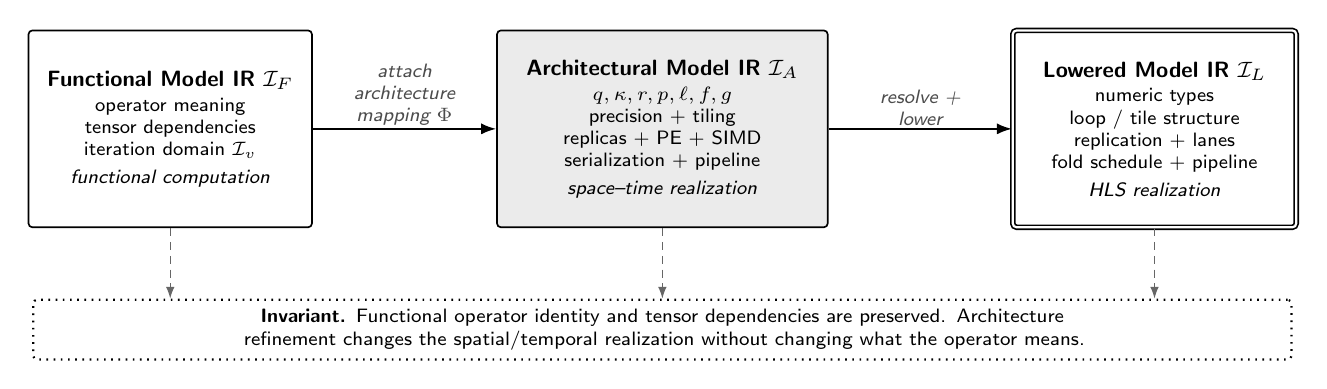
\begin{tikzpicture}[x=1cm,y=1cm]
  \node[sem,minimum width=3.60cm,minimum height=2.5cm] (fun) at (1.80,1.55)
    {\ft{Functional Model IR $\mathcal{I}_F$}\\[1pt]operator meaning\\tensor dependencies\\iteration domain $\mathcal{I}_v$\\[2pt]\emph{functional computation}};
  \node[arch,minimum width=4.20cm,minimum height=2.5cm] (arch) at (8.05,1.55)
    {\ft{Architectural Model IR $\mathcal{I}_A$}\\[1pt]$q,\kappa,r,p,\ell,f,g$\\precision + tiling\\replicas + PE + SIMD\\serialization + pipeline\\[2pt]\emph{space--time realization}};
  \node[phys,minimum width=3.60cm,minimum height=2.5cm] (low) at (14.30,1.55)
    {\ft{Lowered Model IR $\mathcal{I}_L$}\\[1pt]numeric types\\loop / tile structure\\replication + lanes\\fold schedule + pipeline\\[2pt]\emph{HLS realization}};

  \draw[flow] (fun)--node[elab,above]{attach\\architecture\\mapping $\Phi$}(arch);
  \draw[flow] (arch)--node[elab,above]{resolve +\\lower}(low);

  \node[evidence,text width=15.70cm] (prov) at (8.05,-1.00)
    {\textbf{Invariant.} Functional operator identity and tensor dependencies are preserved. Architecture refinement changes the spatial/temporal realization without changing what the operator means.};
  \draw[meta] (fun.south)--(fun.south |- prov.north);
  \draw[meta] (arch.south)--(arch.south |- prov.north);
  \draw[meta] (low.south)--(low.south |- prov.north);
\end{tikzpicture}
\caption{Progressive refinement of one Model IR. Functional meaning remains stable while an explicit space--time architecture mapping is attached and subsequently lowered into HLS-ready mechanisms.}
\label{fig:progressive-ir}
\end{figure*}

\paragraph{Spatial and temporal coordinates.}
\label{sec:spacetime}


The numerical representation $q_v(i)$ determines the arithmetic interpretation used for the corresponding logical work. For example, the architecture representation admits width and format selections such as 8, 12, or 16 bits; these examples do not constitute a new qualified precision sweep. FPGAI does not introduce a PTQ or QAT method; it evaluates whether the selected representation preserves the required numerical behavior and how it changes physical cost.

For reference tensor $x$ and compiled observation $\hat{x}$,
\begin{align}
\operatorname{RMSE}(x,\hat{x})
&=
\sqrt{\frac{1}{N}\sum_{j=1}^{N}(x_j-\hat{x}_j)^2},\\
E_{\max}(x,\hat{x})
&=
\max_j |x_j-\hat{x}_j|.
\end{align}
A cheaper numerical representation that violates the declared numerical acceptance criterion is not considered a valid architecture point.


The mapping $r_v(i)$ assigns logical work to a coarse replica or independently active work group. Coarse parallelism can represent, for example, independently processed tiles, output groups, or replicated operator instances. It is intentionally distinct from PE and SIMD structure.

If the number of active replicas is bounded by requested parallelism $P_v$,
\begin{equation}
|\operatorname{range}(r_v)|\le P_v.
\label{eq:coarse-par}
\end{equation}


The mapping $p_v(i)$ assigns work to processing elements. A PE is an operator-local spatial compute structure with a stable semantic role defined by the selected implementation. For a dense layer a PE may own one or more output-neuron groups; for matrix multiplication it may own rows, columns, or tiles; for convolution it may correspond to output-channel or spatial groups.

The cardinality constraint is
\begin{equation}
|\operatorname{range}(p_v)|\le N_{\mathrm{PE},v}.
\label{eq:pe-cardinality}
\end{equation}
The PE interpretation is part of the operator implementation contract and must be explicit; a value such as $N_{\mathrm{PE}}=4$ is not meaningful if the compiler cannot state what is replicated four times.


The mapping $\ell_v(i)$ assigns work to SIMD lanes within a PE:
\begin{equation}
|\operatorname{range}(\ell_v)|\le N_{\mathrm{SIMD},v}.
\label{eq:simd-cardinality}
\end{equation}
SIMD therefore expresses lane-level arithmetic concurrency rather than independent PE-level concurrency.

A simplified declared spatial width is
\begin{equation}
W_{\mathrm{decl}}
=
P_v
N_{\mathrm{PE},v}
N_{\mathrm{SIMD},v},
\label{eq:decl-width}
\end{equation}
but Eq.~\ref{eq:decl-width} is not treated as a performance law. Dependencies, memory access, routing, resource packing, and pipeline feasibility can prevent linear speedup.


The mapping $f_v(i)$ identifies the temporal reuse or folding step at which work executes on an assigned spatial structure. Serialization is therefore not merely ``less parallelism'': it is an explicit mapping of multiple logical operations onto reused hardware across time.

For two distinct logical iterations $i\neq j$, if they occupy the same exclusive spatial execution coordinate,
\begin{equation}
\sigma_v(i)=\sigma_v(j),
\label{eq:same-resource}
\end{equation}
and the selected implementation does not permit the corresponding operations to issue simultaneously on that resource, then their temporal assignments must be distinct,
\begin{equation}
\tau_v(i)\neq\tau_v(j).
\label{eq:serialization-legality}
\end{equation}
The backend-specific schedule refines $\tau_v$ into concrete cycle-level issue times. Equations~\ref{eq:same-resource}--\ref{eq:serialization-legality} therefore express collision freedom at the portable architecture level without assuming one universal microarchitecture.


The tile mapping $\kappa_v$ partitions or covers the logical iteration domain:
\begin{equation}
\mathcal{I}_v
=
\bigcup_{\theta\in\Theta_v}
\mathcal{I}_{v,\theta},
\label{eq:tile-cover}
\end{equation}
where $\Theta_v$ is the set of tiles. If tiles are intended to be non-overlapping,
\begin{equation}
\mathcal{I}_{v,\theta_1}
\cap
\mathcal{I}_{v,\theta_2}
=
\varnothing
\qquad
(\theta_1\neq\theta_2).
\label{eq:tile-disjoint}
\end{equation}

For matrix multiplication, a tile can be parameterized by
\begin{equation}
T=(T_M,T_N,T_K).
\end{equation}
For convolution, tile dimensions can refer to output channels, input channels, spatial coordinates, and kernel loops. Non-divisible dimensions require explicit tail, mask, or padding semantics; silent truncation is illegal.


The mapping $g_v(i)$ describes the pipeline execution relation for logical work. FPGAI distinguishes an architecture request for overlap from the physical result achieved by the HLS tool.

For a functional dependence $i\prec_G j$ with effective latency $\lambda(i)$, a legal schedule, which assigns each iteration a cycle-level issue time $t(\cdot)$ refining $\tau_v$, must satisfy
\begin{equation}
t(j)\ge t(i)+\lambda(i),
\label{eq:dependency-preservation}
\end{equation}
under the selected implementation semantics.

Where initiation interval is meaningful, an architectural request may specify
\begin{equation}
II_{\mathrm{req}}\ge 1.
\end{equation}
The compiler may emit an HLS pipeline request, but the architecture is reported as successfully realized only if later evidence establishes the effective schedule/II consistent with the claim being made.

\begin{figure*}[t]
\centering
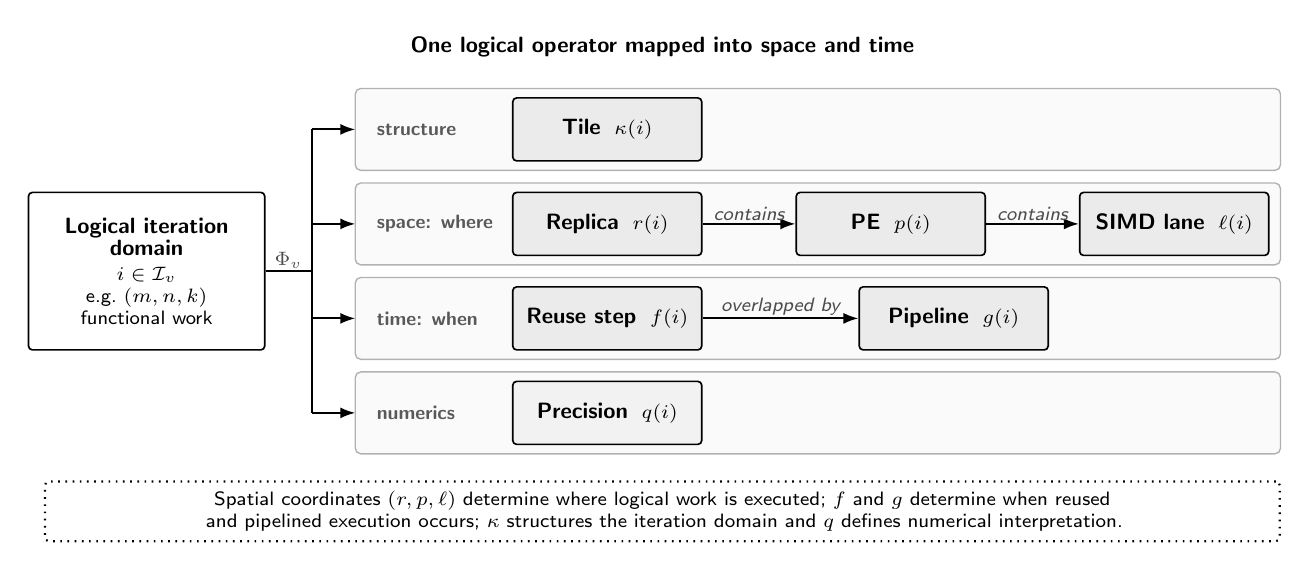
\begin{tikzpicture}[x=1cm,y=1cm]
  \node[ttl] at (8.10,3.45) {One logical operator mapped into space and time};

  % Logical work (functional).
  \node[sem,minimum width=3.00cm,minimum height=2.00cm] (domain) at (1.55,0.60)
    {\ft{Logical iteration}\\\ft{domain}\\[1pt]$i\in\mathcal{I}_v$\\e.g.\ $(m,n,k)$\\functional work};

  % Four roles of the mapping, one lane each.
  \foreach \y/\lab in {2.40/{structure},1.20/{space: where},0.00/{time: when},-1.20/{numerics}} {
    \draw[black!30, line width=0.5pt, rounded corners=2pt, fill=black!2] (4.20,\y-0.52) rectangle (15.95,\y+0.52);
    \node[font=\sffamily\scriptsize\bfseries, text=black!65, anchor=west] at (4.35,\y) {\lab};
  }
  \node[arch,minimum width=2.40cm,minimum height=0.80cm] (tile) at (7.40,2.40) {\ft{Tile} \ $\kappa(i)$};
  \node[arch,minimum width=2.40cm,minimum height=0.80cm] (rep)  at (7.40,1.20) {\ft{Replica} \ $r(i)$};
  \node[arch,minimum width=2.40cm,minimum height=0.80cm] (pe)   at (11.00,1.20) {\ft{PE} \ $p(i)$};
  \node[arch,minimum width=2.40cm,minimum height=0.80cm] (lane) at (14.60,1.20) {\ft{SIMD lane} \ $\ell(i)$};
  \node[arch,minimum width=2.40cm,minimum height=0.80cm] (fold) at (7.40,0.00) {\ft{Reuse step} \ $f(i)$};
  \node[arch,minimum width=2.40cm,minimum height=0.80cm] (pipe) at (11.80,0.00) {\ft{Pipeline} \ $g(i)$};
  \node[contract,minimum width=2.40cm,minimum height=0.80cm] (prec) at (7.40,-1.20) {\ft{Precision} \ $q(i)$};

  \draw[flow] (rep)--node[elab,above]{contains}(pe);
  \draw[flow] (pe)--node[elab,above]{contains}(lane);
  \draw[flow] (fold)--node[elab,above]{overlapped by}(pipe);

  % Mapping Phi_v fans out from the iteration domain to every lane.
  \draw[line width=0.7pt] (domain.east) -- (3.65,0.60);
  \draw[line width=0.7pt] (3.65,-1.20) -- (3.65,2.40);
  \foreach \y in {2.40,1.20,0.00,-1.20} \draw[flow] (3.65,\y) -- (4.20,\y);
  \node[elab,above] at (3.35,0.60) {$\Phi_v$};

  \node[evidence,text width=15.40cm] at (8.10,-2.45)
    {Spatial coordinates $(r,p,\ell)$ determine where logical work is executed; $f$ and $g$ determine when reused and pipelined execution occurs; $\kappa$ structures the iteration domain and $q$ defines numerical interpretation.};
\end{tikzpicture}
\caption{FPGAI space--time architecture mapping. The seven user-visible architecture dimensions are represented as components of one operator mapping rather than as unrelated backend flags.}
\label{fig:spacetime}
\end{figure*}

\paragraph{Architecture resolution and legality.}
\label{sec:resolution}

A useful architecture IR must represent not only valid designs but also why a requested design is invalid. Let $A_{\mathrm{req}}$ denote the requested architecture for graph $G$ and target $D$. FPGAI resolves
\begin{equation}
\Phi^\star
=
\operatorname{Resolve}(G,A_{\mathrm{req}},D).
\label{eq:resolve-main}
\end{equation}

The result is either a legal effective mapping,
\begin{equation}
\Phi^\star\models A_{\mathrm{req}},
\end{equation}
or an explicit blocker
\begin{equation}
\Phi^\star=\bot_{A}.
\end{equation}


Every logical iteration must be represented:
\begin{equation}
\forall i\in\mathcal{I}_v:
\Phi_v(i)\ \text{is defined}.
\label{eq:coverage}
\end{equation}
This prevents an architecture transformation from silently dropping work.


Replica, PE and SIMD cardinalities must satisfy Eqs.~\ref{eq:coarse-par}, \ref{eq:pe-cardinality} and \ref{eq:simd-cardinality}. Additional implementation-specific capacity constraints can be attached to the operator realization.


Iterations mapped to the same exclusive spatial resource must not occupy the same incompatible temporal slot. Equation~\ref{eq:serialization-legality} provides the basic form; operator implementations may refine this when one resource can execute multiple operations per cycle.


The resolved schedule must preserve functional dependencies. Equation~\ref{eq:dependency-preservation} is the basic condition. Pipelining may overlap independent or properly staged work, but cannot change the model's required dependence ordering.


Tile domains must satisfy coverage and the intended overlap/disjointness rules. Boundary behavior for non-divisible dimensions must be explicit.


Let
\begin{equation}
R(\Phi,G,D)
=
(R_{\mathrm{LUT}},R_{\mathrm{FF}},R_{\mathrm{DSP}},R_{\mathrm{BRAM}},\ldots)
\end{equation}
denote resource demand as observed later or an explicitly declared approximation, when available. A feasible candidate must satisfy
\begin{equation}
R_k(\Phi,G,D)\le C_k(D)
\qquad
\forall k
\label{eq:resource-feasibility}
\end{equation}
for enforced device capacities $C_k(D)$.

For the bounded source-level decision study, only declared source constraints are used as admission predicates; no actual physical resource estimator is assumed. Separately measured HLS and routed capacities cannot be inferred from the source bound. Final physical evidence remains a separate stage. For experimental reporting, admissibility is evidence-level dependent. Let $\mathcal{Q}_E$ be the checks required by a specific stage $E$; the set contains numerical equivalence only at stages that actually exercise numerical behavior, and physical timing and design-rule checks only when implementation evidence is available. We write
\begin{equation}
\operatorname{Valid}_{E}(A)=\bigwedge_{q\in\mathcal{Q}_E}q(A),
\label{eq:validity-predicate}
\end{equation}
where each unmeasured required predicate has status \emph{unknown}, never implicitly true. Therefore source certification does not imply HLS timing feasibility, and HLS scheduling estimates cannot be promoted to routed setup/hold closure or board performance.


The requested architecture is not assumed to equal the effective architecture. Let
\begin{equation}
A_{\mathrm{eff}}
=
\operatorname{Project}(\Phi^\star)
\end{equation}
be the effective architecture summary derived from the resolved mapping.

This distinction leads to target-relative architecture equivalence for requests that resolve to legal mappings:
\begin{equation}
A_1
\equiv_{G,D}
A_2
\iff
\operatorname{Resolve}(G,A_1,D)
=
\operatorname{Resolve}(G,A_2,D).
\label{eq:architecture-equivalence}
\end{equation}
Two syntactically different requests that resolve to the same mapping therefore represent one effective architecture point, not two independent physical designs.

\begin{figure*}[t]
\centering
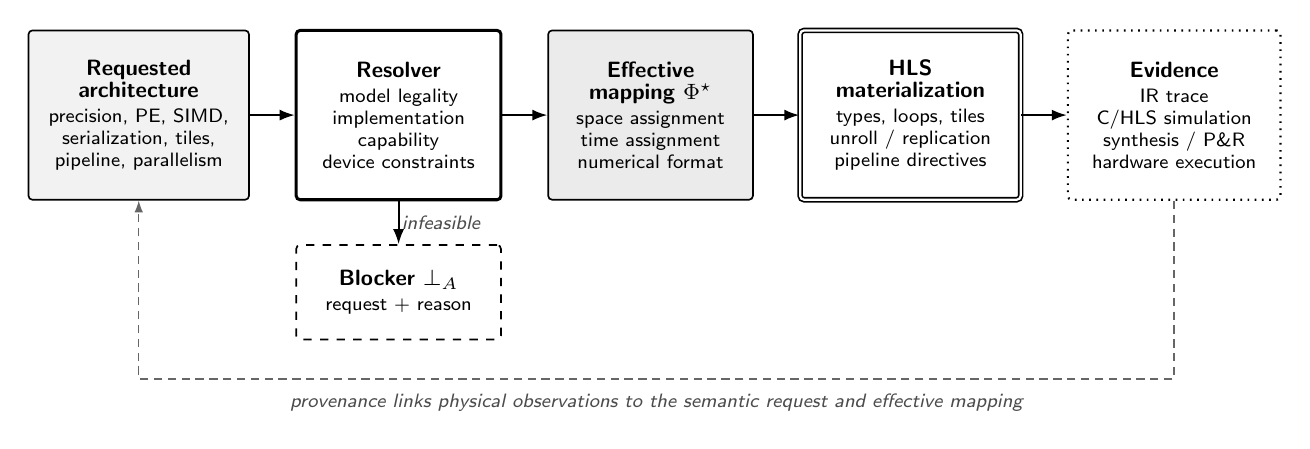
\begin{tikzpicture}[x=1cm,y=1cm]
  \node[contract,minimum width=2.80cm,minimum height=2.15cm] (req) at (1.40,0)
    {\ft{Requested}\\\ft{architecture}\\[1pt]precision, PE, SIMD,\\serialization, tiles,\\pipeline, parallelism};
  \node[stage,minimum width=2.60cm,minimum height=2.15cm] (res) at (4.70,0)
    {\ft{Resolver}\\[1pt]model legality\\implementation\\capability\\device constraints};
  \node[arch,minimum width=2.60cm,minimum height=2.15cm] (eff) at (7.90,0)
    {\ft{Effective}\\\ft{mapping $\Phi^\star$}\\[1pt]space assignment\\time assignment\\numerical format};
  \node[phys,minimum width=2.80cm,minimum height=2.15cm] (hls) at (11.20,0)
    {\ft{HLS}\\\ft{materialization}\\[1pt]types, loops, tiles\\unroll / replication\\pipeline directives};
  \node[evidence,minimum width=2.70cm,minimum height=2.15cm] (ev) at (14.55,0)
    {\ft{Evidence}\\[1pt]IR trace\\C/HLS simulation\\synthesis / P\&R\\hardware execution};

  \draw[flow] (req)--(res);
  \draw[flow] (res)--(eff);
  \draw[flow] (eff)--(hls);
  \draw[flow] (hls)--(ev);

  \node[derived,minimum width=2.60cm,minimum height=1.20cm] (block) at (4.70,-2.25)
    {\ft{Blocker $\bot_A$}\\[1pt]request + reason};
  \draw[flow] (res.south)--node[elab,right]{infeasible}(block.north);

  \draw[meta] (ev.south)--(14.55,-3.35)--(1.40,-3.35)--(req.south);
  \node[note,anchor=north] at (7.975,-3.42)
    {provenance links physical observations to the semantic request and effective mapping};
\end{tikzpicture}
\caption{Architecture resolution and experimental accountability. FPGAI distinguishes requested architecture, effective space--time mapping, HLS materialization, and physical evidence.}
\label{fig:resolution}
\end{figure*}

\paragraph{Scoped architecture decisions.}
\label{sec:scope}

A flat global parameter set is insufficient because different operators can require different spatial and temporal organizations. FPGAI therefore supports scoped architecture semantics.

Let $\mathcal{S}$ denote the ordered set of scopes used in this paper:
\begin{equation}
\mathcal{S}
=
\{
s_{\mathrm{model}},
s_{\mathrm{region}},
s_{\mathrm{op}},
s_{\mathrm{loop}}
\}.
\label{eq:scopes}
\end{equation}
For architecture property $a$ and object $x$, the effective request is obtained by a property-specific resolution function
\begin{equation}
a_{\mathrm{req}}(x)
=
\mathcal{R}_a
\left(
a_{\mathrm{model}},
a_{\mathrm{region}},
a_{\mathrm{op}},
a_{\mathrm{loop}}
\right).
\label{eq:scope-resolution}
\end{equation}

The function $\mathcal{R}_a$ is not assumed to be simple textual override. A local PE request may refine a model default, while a resource constraint can restrict rather than replace lower-level choices. The important property is that the source scope of each effective architectural decision remains identifiable.

For example, a model may request 12-bit precision and two PEs by default, while a dominant GEMM operator requests eight PEs, four SIMD lanes, a specific $(T_M,T_N,T_K)$ tile, and target $II=1$. The effective mapping is resolved for the local operator while preserving the origin of each value.

Backend-local implementation details remain distinct. A compiler-generated loop variable, a particular HLS pragma spelling, or an implementation-specific loop interchange is not automatically promoted to portable architecture semantics. It becomes evidence of a semantic request only through the lowering provenance chain.

\paragraph{Lowering to synthesizable source.}
\label{sec:hls}

The HLS backend consumes $\mathcal{I}_{L}$ rather than reading user-facing architecture configuration directly. This separation prevents the HLS emitter from silently becoming the semantic resolver.

A resolved architecture is materialized through a set of backend mechanisms whose relation to the semantic mapping remains explicit. The numerical component $q$ becomes a fixed-width or fixed-point HLS/C++ representation. The tiling component $\kappa$ becomes explicit tile loops, local bounds, and boundary handling. Coarse parallelism $r$ becomes replicated operator or work-group structures, while the PE mapping $p$ becomes replicated PE compute structures or PE-indexed loop partitions. The lane mapping $\ell$ becomes vectorized or unrolled inner arithmetic, temporal reuse $f$ becomes folded loops and reuse schedules, and the pipeline relation $g$ becomes pipeline staging together with HLS pipeline or initiation-interval directives where the selected implementation supports them. These lowerings are implementation mechanisms for the resolved semantics rather than independent architecture decisions.

Different HLS source encodings may be equivalent realizations of the same architecture semantics. Therefore FPGAI does not define architecture by one particular pragma or source template. The backend must instead satisfy the resolved mapping:
\begin{equation}
\operatorname{EmitHLS}(\mathcal{I}_{L})
\models
\Phi^\star.
\label{eq:hls-satisfies}
\end{equation}

If generated source requests $II=1$ but synthesis reports a larger achieved initiation interval, the request and observation are kept distinct. Emitting a directive is source-level evidence of intent; satisfying that request is a separately established synthesis or implementation result.

\section{Source Contracts and Executable Checking}
\label{sec:sourcecontracts}
\paragraph{Finite operational semantics.}
For the admitted static source families, define a finite typed tensor-element value $v=(\text{tensor},\text{index})$ and its expected producer contributions $\operatorname{Terms}(v)$ and required consumer tokens $\operatorname{Use}(v)$. The supported event alphabet is
\begin{align}
\operatorname{CONTRIBUTE}(v,k)&\quad\text{a unique producer reduction term},\\
\operatorname{COMMIT}(v)&\quad\text{completed element becomes readable},\\
\operatorname{READ}(v,c)&\quad\text{declared consumer $c$ reads element $v$}.
\label{eq:events}
\end{align}
A finite source trace $e_0,e_1,\ldots,e_{m-1}$ is interpreted by a partial operational transition system. The interpreter state consists of the set $\mathrm{Com}$ of committed values, observed terms $K(v)$, observed consumers $\mathrm{Rd}(v)$, and a partial live-address map $\mathrm{Occ}:\text{scratch address}\rightharpoonup\text{value}$.

An event is admissible only if its tensor/consumer identity and indices are well formed and the following obligations hold: a contribution has a new expected reduction index; a commit follows all required producer terms (or completion of its required incoming reads); a read is by a unique declared consumer after commit while the address holds exactly that value; and the scratch slot is released only after $\mathrm{Rd}(v)=\operatorname{Use}(v)$. Distinct checks validate expected operator-specific $\Phi$ ownership and the supported source issue-order relation. Event acceptance is defined by \emph{all} relevant checks, not just a numeric output check.

\begin{figure}[t]
\centering
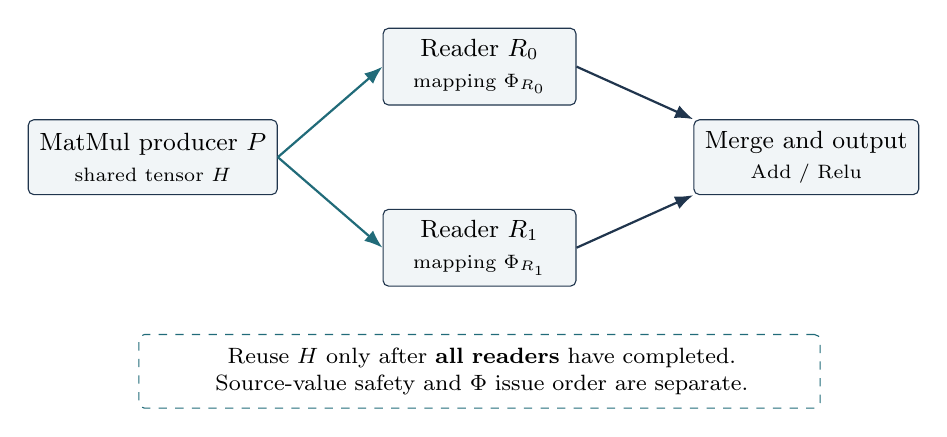
\begin{tikzpicture}[x=1cm,y=1cm,>=Latex,
 block/.style={draw=navy,rounded corners=2pt,fill=pale,
 minimum width=2.45cm,minimum height=0.95cm,align=center,inner sep=4pt,font=\small}]
\node[block] (p) at (0,1.20) {MatMul producer $P$\\\scriptsize shared tensor $H$};
\node[block] (a) at (4.15,2.35) {Reader $R_0$\\\scriptsize mapping $\Phi_{R_0}$};
\node[block] (b) at (4.15,0.05) {Reader $R_1$\\\scriptsize mapping $\Phi_{R_1}$};
\node[block] (m) at (8.30,1.20) {Merge and output\\\scriptsize Add / Relu};
\draw[->,thick,darkteal] (p.east) -- (a.west);
\draw[->,thick,darkteal] (p.east) -- (b.west);
\draw[->,thick,navy] (a.east) -- (m.north west);
\draw[->,thick,navy] (b.east) -- (m.south west);
\node[draw=darkteal,dashed,rounded corners=2pt,fill=white,
 text width=8.3cm,align=center,font=\footnotesize,
 inner sep=5pt] at (4.15,-1.52)
 {Reuse $H$ only after \textbf{all readers} have completed.\\
 Source-value safety and $\Phi$ issue order are separate.};
\end{tikzpicture}
\caption{Bounded multi-reader source contract. Arrows represent typed tensor dependencies, not hardware-cycle memory-port scheduling.}
\label{fig:fanout}
\end{figure}


\begin{proposition}[Source read safety]
Suppose the finite functional model correctly enumerates $\operatorname{Terms}(v)$ and $\operatorname{Use}(v)$ for every supported value, and the event interpreter accepts a trace only when each prefix obeys the operational checks above. Then every accepted $\operatorname{READ}(v,c)$ observes a committed value whose required producer obligations have completed and whose live scratch address still denotes $v$.
\end{proposition}
\noindent\emph{Proof sketch.} Initially no value is committed or live. A contribution only records a new expected term. A commit is admitted only after the complete prerequisite set and when its address is available. A read is admitted only after commit and only for the current live occupant. Induction over trace prefixes establishes the stated property. This proof is conditional on the correctness of the obligation sets and applies to the finite interpreter, not emitted RTL.\par

\begin{proposition}[All-reader source lifetime]
Under the same assumptions, two simultaneously live source values cannot occupy the same scalar scratch address; a slot can be reused only after the last required declared consumer has read the previous occupant.
\end{proposition}
\noindent\emph{Proof sketch.} The live-address map is initially empty. Every admitted commit checks vacancy before adding a binding; only the read completing $\mathrm{Rd}(v)=\operatorname{Use}(v)$ releases it. Induction preserves single occupancy of each slot. This is not a physical BRAM banking, port-concurrency, or clock-domain proof.\par

For one fixed serialized source event order, a scalar value occupies its slot from commit through the last required read. The minimum number of equal-sized scalar slots equals the maximum overlap of these fixed-order intervals. This is a standard interval-coloring property, not a novel theorem; the compiler contribution is the production of the correct bounded intervals from typed model/source events and checking addresses against them. The exact interval bound changes under a hypothetical alternative first-in-place-MAC lifetime convention; this sensitivity is quantified in Section~\ref{sec:results}.

\paragraph{Value safety and issue-order conformance.}
Let $\rho=(e_0,\ldots,e_{m-1})$ be the observed finite source event sequence, let $V_{\mathrm{adm}}\subseteq V$ be the admitted operators, and let $\mathrm{Iss}_v$ denote the admitted set of logical issue tokens for operator $v\in V_{\mathrm{adm}}$. For an issue token $i\in\mathrm{Iss}_v$, the lowering records an expected spatial owner $o_{\Phi_v}(i)$ and a precedence relation $i\prec_{\Phi_v}j$ whenever the mapping requires token $i$ to precede token $j$ in the serialized source order. These are \emph{source} relations: they do not assert an achieved initiation interval or a clock cycle assignment.

An issue token here is the unique declared occurrence of an admitted contribution or read belonging to operator $v$; it is not a fourth event type or a machine cycle. Define $\pi_v(\rho)$ as the projection of the trace onto operator $v$'s issue tokens, including their reported owners. A token is identified by its event label together with its occurrence index, so each token has exactly one position; let $\operatorname{pos}_{\pi_v(\rho)}(i)$ denote that position in the projection. We use the following bounded conformance predicate:
\begin{align}
\operatorname{IssueConform}(\rho,\Phi)\;\Longleftrightarrow\;
\bigwedge_{v\in V_{\mathrm{adm}}}\Big[&
\operatorname{Tokens}(\pi_v(\rho))=\mathrm{Iss}_v\;\wedge\label{eq:issue-conform}\\[-2pt]
&\bigwedge_{i\in\mathrm{Iss}_v}\operatorname{owner}_\rho(i)=o_{\Phi_v}(i)\;\wedge\notag\\[-2pt]
&\bigwedge_{i\prec_{\Phi_v}j}
\operatorname{pos}_{\pi_v(\rho)}(i)<\operatorname{pos}_{\pi_v(\rho)}(j)\Big].\notag
\end{align}
Here equality of token sets includes their prescribed multiplicities. In fully serialized schedules, $\prec_{\Phi_v}$ is the prescribed source order; when the admitted mapping leaves independent tokens unordered, the predicate does not impose an arbitrary total order. The bounded compiler checker builds the expected tokens and source order from the selected operator mapping, not from a physical schedule inferred by Vitis HLS.

The source contract is therefore
\begin{equation}
\operatorname{SourceContract}(\rho,\Phi)
=\operatorname{SafeValues}(\rho)\land\operatorname{IssueConform}(\rho,\Phi),
\label{eq:contract}
\end{equation}
where $\operatorname{SafeValues}(\rho)$ checks required contribution completion, unique declared reads and nonaliasing of simultaneously live scalar values. A program can satisfy value safety and preserve its output while violating $\operatorname{IssueConform}$: swapping otherwise safe reader issues is a counterexample whenever the corresponding precedence edge is required by the declared mapping. This construction states the property tested by the order mutants and shows that the checker is not merely another numerical comparison.


An abstract certificate is not automatically a certificate for generated C++. For the bounded generated source family, we instrument actual scratch loads and stores with a dynamic owner map and compare them against the source events and storage addresses. An adversarial mutation changes the \emph{actual} C++ memory address while leaving the printed source witness unchanged. Thus a test that trusts the printed address alone would miss the actual access mismatch, whereas the instrumented source check can observe it. The invariant checked during host execution is that, after a committed write to address $a(v)$ and before its last required read, no different live value overwrites $a(v)$ and each read obtains the declared occupant. The instrumentation is an executable source-level check, not hardware memory port verification.

In the emitted source experiment, six unmodified host programs passed their baseline checks. Thirty-six distinct source mutants were applied to each of six bounded graphs, drawn from nine mutation families with four variants each. Eight families alter an actual scratch load or store (shifted store or load indices for the producer, reader, Add and final-activation accesses, and a suppressed producer store whose commit is still printed), giving 32 memory-operation mutants per graph; the ninth perturbs the producer arithmetic, giving four arithmetic mutants per graph. All 216 selected mutants were detected. The aggregate audit reports 192 detections by the dynamic scratch shadow and 24 by the original source checker; the fault population separately contains 192 memory-operation variants and 24 arithmetic variants. These equal totals should not be interpreted as a verified family-by-detector cross-tabulation without the original per-mutant outcome file. No mutant survived, failed to compile, or ended in an unexplained state in that fixed campaign. This establishes detection adequacy for the selected mutation classes under the original compiler revision, not an all input proof of emitted source refinement or a competitor comparison.


The two prefix safety propositions are conditional on complete $\operatorname{Terms}(v)$ and $\operatorname{Use}(v)$ declarations for the admitted static matrix product source family. Both finite event interpreters share those declared graph obligations. The issued source trace, host C++ execution, HLS schedule and placed FPGA circuit therefore remain separate objects of evidence. In particular, the current contract does not establish arbitrary neural graph soundness, physical RAM port feasibility, clock-domain crossing or a cycle-accurate pipeline schedule.

\section{Policy-Independent Architecture Decisions}
\label{sec:decisions}

A complete source design state contains a functional graph, a request for each operator, an exchange/layout selection, and explicit source target limits:
\begin{equation}
S=(F,A,X,L),\qquad a=(\mathsf{scope},\mathsf{target},\mathsf{field},\mathsf{value}).
\label{eq:state}
\end{equation}
The compiler returns a non-mutating transition outcome
\begin{equation}
\mathcal{T}(S,a)\in\{\reject,\unknown,\cert\}.
\label{eq:transition}
\end{equation}
A successful source lowering also returns a typed next-state receipt; rejection preserves $S$. The $\unknown$ status means the source was admitted but its bounded ownership obligations were \emph{not} certified. It cannot be promoted to acceptance. The $\cert$ status attests only to a source contract in the supported domain. None of the three results predicts FPGA timing or physical feasibility.

For a finite declared candidate catalog $C=(a_1,\ldots,a_n)$, the mask is
\begin{equation}
\mathcal{M}_{\src}(S,C)_i
=\mathbf 1\bigl[\mathcal{T}(S,a_i)=\cert\bigr].
\label{eq:mask}
\end{equation}
The mask calls the \emph{ordinary source compiler} on every candidate. It is therefore compiler-relative, policy-independent, and conservative with respect to uncertified source status; it is not a separate learned approximation to HLS performance.


The interface exposes a variable-size typed graph observation $\Omega(S)$ with operator/tensor identities in a structured schema, operator types, shapes, mapping/target attributes and source-domain properties. It does not expose raw tensor weights, previous rewards or a trained policy's hidden state. Supported observations preserve their public features under consistent source-node renaming and node/edge-list ordering. A structural hash invariant under those permutations is a \emph{fingerprint of available features}: relabelled copies of the same typed graph receive the same hash, but equal hashes do not prove isomorphism, and functionally equivalent models with different public structure are not identified. The decision interface remains usable by enumeration, a heuristic, a human or a future RL policy.


The policy-independent compiled-once catalog retains the source-attested typed next state for each candidate. If a candidate is already $\cert$, it can be selected and returned from the in-process immutable catalog without a second source compiler transition. A rejected or unknown candidate cannot be selected as certified, and a cached transition is bound to the original source-state identity. Crucially, this saves \emph{an additional transition after screening}: constructing a catalog of $n$ candidates still requires $n$ compiler transitions. It may be less efficient than compiling one blind proposal; no general exploration speedup is inferred.

\begin{figure}[t]
\centering
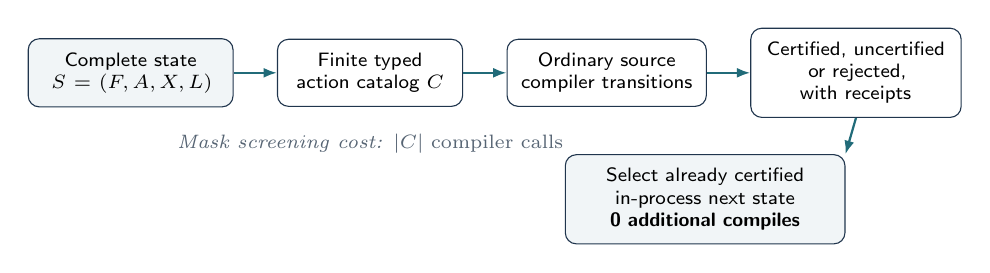
\begin{tikzpicture}[node distance=0.52cm, font=\footnotesize,
 nodebox/.style={draw=navy,rounded corners,align=center,minimum height=0.75cm,inner sep=5pt},
 arrow/.style={-{Latex[length=1.7mm]},thick,darkteal}]
\node[nodebox,fill=pale,text width=2.25cm] (s) {Complete state\\$S=(F,A,X,L)$};
\node[nodebox,right=0.55cm of s,text width=2.00cm] (c) {Finite typed\\action catalog $C$};
\node[nodebox,right=0.55cm of c,text width=2.18cm] (t) {Ordinary source\\compiler transitions};
\node[nodebox,right=0.55cm of t,text width=2.32cm] (o) {Certified, uncertified\\or rejected, with receipts};
\draw[arrow] (s)--(c);\draw[arrow] (c)--(t);\draw[arrow] (t)--(o);
\node[nodebox,below=0.60cm of t,xshift=1.25cm,fill=pale,text width=3.2cm] (pick) {Select already certified\\in-process next state\\\textbf{0 additional compiles}};
\draw[arrow] (o.south)--(pick.north east);
\node[below=0.22cm of c,font=\scriptsize,text=muted,align=center]{\emph{Mask screening cost:} $|C|$ compiler calls};
\end{tikzpicture}
\caption{Policy-independent compiler actions and cached selection. Screening requires one ordinary compiler transition per proposed source candidate; certification is restricted to the supported source contract.}
\label{fig:c2}
\end{figure}

\section{Experimental Design}
\label{sec:method}

The experiments are fixed finite populations rather than randomly sampled model sets. We use the following evidence distinctions. \emph{Source semantics} checks typed events and allocation; \emph{host execution} checks original generated C++ operations and their numerical or address witnesses; \emph{native C simulation} evaluates the HLS testbench; \emph{HLS synthesis} yields estimated resource and cycle reports subject to the specified timing criterion; and \emph{routed implementation} supplies target-specific utilization, design-rule and worst-negative-slack observations. These categories must not be promoted into one another.

\begin{table}[H]
\centering
\caption{Study populations, architectural interventions, and evidence criteria.}
\label{tab:setup}
\small
\renewcommand{\arraystretch}{1.15}
\setlength{\tabcolsep}{4pt}
\begin{tabularx}{\linewidth}{@{}>{\raggedright\arraybackslash}p{3.35cm}>{\raggedright\arraybackslash}X>{\raggedright\arraybackslash}p{3.65cm}@{}}
\toprule
Population and size & Comparison or intervention & Measurement stage \\
\midrule
Tensor semantics and generated source & Finite allocation oracles, event perturbations, and injected C++ memory and arithmetic faults & Separate event interpretation and host C++ execution \\
Memory layout: 32 designs & Two fanout graphs, four binary factors, 64 matched contrasts & Vitis HLS simulation and synthesis \\
Neural networks: 6 designs & Three functional topologies, each with scalar and independently mapped architectures & Vitis HLS simulation and synthesis \\
MNIST architectures: 8 designs & Four architecture mappings for each of an MLP and a CNN & Earlier out-of-context routed timing \\
Recent storage-clock pilot: 6 routes & Full/row source storage, each at 16, 20 and 24~ns; reused earlier HLS RTL & Routed setup slack, utilization and DRC status, descriptive only \\
\bottomrule
\end{tabularx}
\tablenote{Both original HLS cohorts used the AMD 2023.2 toolchain context. The memory study specified an 8~ns clock with 1.5~ns uncertainty and numerical C-simulation tolerance 0.01; the neural-network study specified 10~ns with 1~ns uncertainty. Earlier MNIST target/constraint records were insufficient for independent reconstruction. The subsequent six-route pilot and four prepared storage--pipeline source cases are separate from all earlier denominators; neither supplies clean-DRC physical or board latency evidence.}
\end{table}

The source packages and report hashes, not just an exit status, determine the identity of a native measurement. The HLS toolchain configuration used by the research pipeline defaults to part \texttt{xck26-sfvc784-2LV-c}; because the complete original vendor manifests are not redistributed with this manuscript, we do not substitute that default for independently inspecting every original case's recorded part. The HLS estimated period is compared with the \emph{effective} time budget after the declared uncertainty. The failure of the convolution and dense strided pair at 9.181 ns is thus 0.181 ns beyond 9.000 ns, rather than a failed post-route WNS measurement.


We use static MatMul chains and fanout graphs with two to four readers, selected additions and activation stages. Five small fixed-order scalar slot instances are compared with an independent exhaustive oracle. Twenty-five selected adverse event mutations test premature reads, incomplete accumulation, owner or issue-order errors and live address overlap. A separate interpreter comparison evaluates 133 canonical and mutated source traces. Both interpreters use the same static graph specification, so agreement tests implementation consistency rather than an independent specification theorem.

A later host-executed conformance cohort holds the underlying bounded graph family and canonical events fixed over 54 configurations varying two to four readers and scalar or mixed operator mappings. Each graph is materialized as both disjoint source storage and fixed-order per-element reused storage, yielding 108 actual generated-C++ GCC executions. This population tests whether an allocation satisfying the finite source obligations can be materialized without losing the matched output and access witnesses. It does not provide a separate sample of 54 independent real-world applications or physical FPGA implementations.

The generated source intervention uses six graph instances, each with one unmodified host baseline and 36 deliberately altered C++ programs. Eight of the nine mutation families perturb scratch stores and loads (producer, reader, Add and final-activation accesses, including one suppressed store); the ninth perturbs producer arithmetic. Source code and outcome files are associated with the original source revision and their own hashes. A mutant that fails to compile is not credited as a detection. The reported original campaign has 222 executed host programs in total: six baselines and 216 mutations.


For a fixed serialized source order, each scalar value has an interval from its commit to last required read; minimum unit slot count follows the classical maximum overlap bound. The source comparison also evaluates whole tensor contiguous layouts, where tensor elements occupy a single interval and consecutive addresses, and independently verifies 36 finite exact allocation problems. The algorithmic optimum is a source storage comparator, not a new interval coloring theorem and not a prediction of physical BRAM banks or ports.

The downstream HLS study is a complete $2\times 2^4$ design over two shared tensor graph families and four binary source factors: storage layout, address expression, requested memory binding, and array padding. The original 32 native vendor executions have 32 numerical CSim passes and 30 HLS cases satisfying the effective clock criterion. Sixty-four planned conditional one-factor comparisons are evaluated only when both original arms are eligible; the two timing-rejected designs can make a factor comparison unqualified. HLS estimated BRAM18K is the outcome, not routed memory cells. Six earlier Vivado routed memory comparisons are retained separately because their design rule checks were not clean and their original clock protocol differs.


The policy-independent design interface receives a functional graph, architecture mapping, exchange layout and explicit source constraints. One population has six prescribed changes; another has eight complete design edits for each of six graphs, giving 48 compiler transitions. We record rejected, certified and source admitted but uncertified outcomes. Every candidate is evaluated by the ordinary compiler. A previously certified next state may subsequently be selected from a bound immutable catalog without repeating its transition, but constructing that catalog still requires one source compilation per candidate. No trained policy or search quality comparison is included.


The six network HLS cases comprise a convolution--pooling--dense topology, a strided-convolution--dense topology, and a two-convolution--Softmax topology, each under scalar and independently assigned operator mappings. Their workloads use the same synthetic parameters within matched controls and treatments. The completed native campaign includes CSim and HLS synthesis but no matched clean-DRC routed results. A separate, earlier MNIST MLP and CNN comparison records eight out-of-context routed timing observations. Because the available manuscript material does not provide the full device, constraint, report and source bundle for this earlier cohort, we retain its WNS and source equivalence observations as context only; we do not use them to infer achieved board latency, FPGA inference accuracy or a cross cohort performance improvement.


The post-hoc clock feasibility pilot described in Section~\ref{sec:pilot-route} reuses \emph{original HLS-generated RTL} while changing the imposed routed period. It is not an HLS recompilation at the new target period. A separate source-only experiment consequently prepares four \emph{new} 24~ns Vitis source packages for one fixed two-reader MatMul fanout, with the same 1.5~ns HLS uncertainty, numerical input/testbench, target part \texttt{xck26-sfvc784-2LV-c}, and \texttt{ap\_fixed<32,6>} representation. The only factors are full versus row-retained source storage, and no added directive versus an explicitly requested \texttt{PIPELINE II=1} on the canonical producer inner multiply--accumulate loop. The producer request is an intervention on emitted source, not a verified DSP register or achieved initiation interval.

The four new model sources have distinct SHA-256 identities but share a single numerical testbench and HLS Tcl hash. This verifies source-package integrity, not a fresh GCC E1 numerical pass or an E2 C-simulation pass. The source-only audit verified each model and the common numerical-testbench and HLS-constraint files against a frozen source baseline. No new Vitis/Vivado tool was invoked. This establishes a controlled prospective intervention, but it provides no fresh numerical C-simulation, HLS scheduling, routed hardware, or board-level latency observation. Its results are consequently excluded from all hardware-performance contrasts reported below.


Each experimental population was executed under a separately fixed source revision and retains its own generated source, input, and observation identity. The original Vitis and host program campaigns are therefore treated as independent cohorts rather than consecutive stages of one hardware experiment. The underlying research ledgers identify the study revisions and observation counts, but the complete generated source, vendor reports, and injected fault programs are not provided with this manuscript. Independent reproduction therefore remains a separate artifact requirement rather than an implied property of the public compiler repository.

\section{Results}
\label{sec:results}
\subsection{Source conformance and generated-program faults}
\begin{table}[H]
\centering
\caption{Verification outcomes for bounded source semantics and emitted C++ operations.}
\label{tab:source-contract-results}
\small
\renewcommand{\arraystretch}{1.15}
\setlength{\tabcolsep}{4.3pt}
\begin{tabularx}{\linewidth}{@{}>{\raggedright\arraybackslash}p{3.40cm}>{\raggedright\arraybackslash}X>{\raggedright\arraybackslash}p{2.18cm}@{}}
\toprule
Verification property & Experimental reference or perturbation & Observed result \\
\midrule
Scalar storage optimality & Independent exhaustive allocator for five source schedules & 5/5 agreement \\
Event contract violations & Twenty-five specified invalid event sequences & 25/25 rejected \\
Event interpreter agreement & 133 original and perturbed finite traces & 133/133 agreement \\
Emitted source baseline & Six unmodified instrumented C++ programs & 6/6 accepted \\
Memory-operation mutants & 32 altered scratch loads or stores for each of six programs & 192/192 detected \\
Arithmetic mutants & 4 perturbed producer computations for each of six programs & 24/24 detected \\
\bottomrule
\end{tabularx}
\tablenote{The aggregate audit reports 192 detections by runtime shadow instrumentation and 24 by the existing source checker. The fault classes separately comprise 192 memory-operation variants and 24 arithmetic variants; a per-mutant detector cross-tabulation is not established here. All instances were deliberately constructed rather than randomly sampled.}
\end{table}

A later independently attested extension linked canonical source events to generated host C++ across matched fanout configurations with different reader counts and operator mappings. Each admitted configuration was executed under a disjoint scratch layout and a fixed-order reuse layout; both layouts passed the selected source-access and numerical checks. Reuse reduced source scratch demand in every admitted configuration, with a median within-program reduction of 50\% and a median saving of 15.5 scalar source slots. Across the distinct programs the recorded capacities summed to 1,999 disjoint versus 1,009 reused slots; these sums are descriptive of separate examples and are not the memory capacity of one deployable accelerator. The largest observed final and intermediate numerical errors were $2.38\times 10^{-7}$ and $2.41\times 10^{-7}$, respectively. This extension comprises 54 source configurations and 108 actual GCC compilations and executions, and is source-level evidence only. The per-element reuse allocator was designed to reduce source slots, so these positive contrasts principally test successful materialization and source conformance rather than a surprising superiority result over independently optimized allocators. The earlier event-mutation population and this host-executed canonical population are separate experiments.

\begin{table}[t]
\centering
\caption{Source scratch-slot reduction in the separately executed GCC fanout cohort. Medians summarize nine fixed profiles in each stratum.}
\label{tab:c1-source-effect}
\small
\setlength{\tabcolsep}{5pt}
\begin{tabularx}{\linewidth}{@{}crrr@{}}
\toprule
Reader mapping & Readers & Median slots saved & Median reduction \\
\midrule
Scalar & 2 & 14 & 45.5\% \\
Mixed $\Phi$ & 2 & 12 & 50.0\% \\
Scalar & 3 & 14 & 50.0\% \\
Mixed $\Phi$ & 3 & 18 & 47.1\% \\
Scalar & 4 & 24 & 50.0\% \\
Mixed $\Phi$ & 4 & 32 & 50.0\% \\
\bottomrule
\end{tabularx}
\tablenote{Unit slots refer to scalar scratch allocation in emitted host source. The selected per-element reuse algorithm is deliberately intended to save slots. These are neither BRAM tiles nor independent FPGA performance samples.}
\end{table}

The generated C++ campaign is the more direct implementation test. Of the 216 mutants, the aggregate audit reports 192 detections by the dynamic shadow that follows the actual scratch addresses passed to loads and stores, and 24 by the existing source checker. The deliberately injected fault population consists of 192 altered memory operations and 24 arithmetic perturbations; a separate per-family detector audit would be required to assign every detection unequivocally to a fault class. All six original programs passed. In particular, a mutant that alters an actual store or load index but leaves the declared trace address unmodified demonstrates why checking a printed source witness alone is insufficient. The experiment detects the selected injected faults within the supported compiler output family. It does not prove that every invalid program is detected, nor that an external compiler lacks an equivalent check.

Separately implemented source event interpretation agreed on 133 trace variants, including adverse reorderings. In the specified five small instances the exhaustive slot reference matched the compiler's fixed-order allocation, and the 25 prescribed faulty event transformations were rejected with their expected source reasons. This supports the implementation of the bounded obligations described in Eq.~\ref{eq:issue-conform}, rather than a theorem about the generated RTL or all possible graphs.


For 27 paired operator mappings, committed-value to last-reader accounting yielded 18 smaller scalar scratch peaks and nine ties. Under a hypothetical first multiply accumulation in place convention the same 27 comparisons yielded \emph{zero} reductions. The choice of lifetime endpoint is therefore part of the modeled source semantics and not an innocuous accounting detail. Separately, an exact finite contiguous tensor allocation analysis solved 36 of 36 fixed source problems; 12 optima improved on a feasible greedy first-fit placement. These counts describe source layout comparisons with specific lifetime constraints. They do not measure BRAM consumption.

\subsection{Source memory allocation and HLS mapping}
\begin{table}[H]
\centering
\caption{Effects of source memory interventions on HLS estimated BRAM18K consumption. Each difference is relative to its matched control.}
\label{tab:hls-factorial}
\small
\renewcommand{\arraystretch}{1.16}
\setlength{\tabcolsep}{3.5pt}
\begin{tabularx}{\linewidth}{@{}Xrrrrr@{}}
\toprule
Contrast population & $n$ & $\Delta<0$ & $\Delta=0$ & $\Delta>0$ & Ineligible \\
\midrule
All factorial contrasts & 64 & 2 & 47 & 8 & 7 \\
Address representation only & 16 & 0 & 14 & 0 & 2 \\
\bottomrule
\end{tabularx}
\tablenote{$\Delta$ is the intervention minus control resource estimate. Of 57 timing-eligible contrasts, 3.5\% decrease, 82.5\% tie, and 14.0\% increase. Address representation is a subset of the 64 contrasts, not an additional population. Eligibility required both arms to satisfy the effective 6.5~ns HLS timing budget. No physical BRAM conclusion is implied.}
\end{table}

All 32 cases passed C simulation, while 30 of 32 satisfied the originally declared HLS effective timing criterion. Among the 64 prespecified one-factor comparisons, 57 are eligible for an estimated BRAM comparison. The eligible results comprise two reductions, 47 ties and eight increases. Both reductions occur in the four-reader source graph; none occurred in the qualified two-reader comparisons. In the eligible address expression contrasts, the HLS BRAM estimate was unchanged in all 14 pairs even though the generated Verilog's static module hierarchy could differ. Two address selection cases that failed the effective HLS timing condition are not treated as resource ties. No native run was repeated to improve this outcome.

Six older matched out-of-context Vivado comparisons likewise reported tied routed BRAM usage. Their reported design rule checks were warning-bearing, so these are \emph{descriptive} routed ties rather than clean qualified physical evidence, and they come from a different HLS source clock protocol. They cannot establish physical resource savings or be pooled numerically with the 32 design HLS factorial. These outcomes show a substantive translation boundary: changing the modeled source lifetime, array layout or address expression often does not change the block memory estimate made by the HLS tool. Potential mechanisms include memory inference, binding, array structure and the available port organization; isolating the cause would require independently qualified netlist and port analysis.

\subsection{Source certification and compiler cost}
\begin{table}[H]
\centering
\caption{Classification of complete architectural proposals by the source semantics verifier.}
\label{tab:decision-results}
\small
\renewcommand{\arraystretch}{1.14}
\setlength{\tabcolsep}{3.6pt}
\begin{tabularx}{\linewidth}{@{}Xrrrr@{}}
\toprule
Functional graph population & Proposals & Certified & Rejected & Uncertified \\
\midrule
Two bounded operator domains & 6 & 3 & 2 & 1 \\
Six chain and fanout graphs & 48 & 21 & 24 & 3 \\
\bottomrule
\end{tabularx}
\tablenote{Certification refers only to the supported source-level tensor and issue-order contract. The populations are separate finite studies and are not treated as a random or additive sample. Evaluating 48 proposals required 48 compiler transitions; selecting an already certified state required no further transition.}
\end{table}

The policy-independent interface was also evaluated in a separate, source-only CPU-cost study using direct compilation, on-demand lazy caching and eager full-catalog construction. For six fixed graph cohorts, multiple deterministic seeds and request patterns produced 108 paired workload conditions, including repeated and cycling requests. Eager preparation lost to lazy caching in every measured paired condition; over the full repeated study, direct, eager and lazy methods performed 1,476, 864 and 198 compiler transitions, respectively. The original eligibility preflight was accounted for separately, and the requests were deliberately restricted to previously certified actions. This is a negative result for an eager screening-cost advantage over lazy reuse, not evidence that all upfront certification is useless: it supplies more complete status information, a benefit not evaluated under blind-action search. Correlated conditions from one fixed graph family must not be treated as independent application replicates.

\begin{table}[t]
\centering
\caption{Median source-compiler wall time (ms) for fixed certified-action request streams. Each row summarizes 18 correlated graph/seed observations, not independent applications.}
\label{tab:c2-screening-cost}
\small
\setlength{\tabcolsep}{5pt}
\begin{tabularx}{\linewidth}{@{}Xrrrr@{}}
\toprule
Request stream & Requests & Direct & Lazy & Eager \\
\midrule
Repeated action & 1 & 9.24 & 9.36 & 36.83 \\
Repeated action & 8 & 73.12 & 9.90 & 38.25 \\
Repeated action & 32 & 293.07 & 12.25 & 42.56 \\
Cycling actions & 1 & 9.19 & 9.30 & 37.25 \\
Cycling actions & 8 & 72.55 & 33.68 & 38.42 \\
Cycling actions & 32 & 290.61 & 36.26 & 43.03 \\
\bottomrule
\end{tabularx}
\tablenote{The 48-call original eligibility preflight is excluded from all timed methods. Each strategy is evaluated against matched certified-only requests; eager catalog construction has the additional information benefit of knowing unqueried action status, which is not valued in this benchmark. Original source study: six graph cohorts, three seeds, two request patterns.}
\end{table}

The larger catalog spans three matrix product chain depths and fanout with two, three and four readers. Every one of its 48 candidates was processed by an actual source compiler transition. The results comprise 21 certified, 24 rejected and three admitted but uncertified states; uncertified actions are excluded from the conservative acceptance mask. The catalog retained source bound typed next states, so selecting an already certified member required no \emph{additional} source compilation after the 48 initial checks. This demonstrates consistency of source action classification and avoidance of redundant recompilation \emph{after} a completed screen. It does not demonstrate a learning-policy benefit, and the independent CPU-cost study finds that eager masking is slower than lazy caching under the measured certified-request workload.

The compiler interface has also been prepared for broader systematic variations of graph shape and source capacity. Those proposed populations are not included in the measured denominators because their executed outcome receipts were not available for verification at the manuscript cutoff.


\begin{table}[H]
\centering
\caption{Numerical qualification and synthesis scheduling in matched neural network architectures.}
\label{tab:neural-hls}
\small
\renewcommand{\arraystretch}{1.15}
\setlength{\tabcolsep}{3.4pt}
\begin{tabularx}{\linewidth}{@{}Xcrrr@{}}
\toprule
Network topology & Eligible & Scalar cycles & Mapped cycles & Cycle ratio \\
\midrule
Convolution, pooling, dense & 2/2 & 624 & 911 & 1.46 \\
Strided convolution, dense & 0/2 & \multicolumn{3}{c@{}}{Timing criterion not met} \\
Two convolutions, softmax & 2/2 & 2,365 & 5,436 & 2.30 \\
\bottomrule
\end{tabularx}
\tablenote{All six designs passed numerical C simulation. The pass fraction denotes synthesis eligibility under a 9.0~ns effective HLS budget, not numerical success. The ratio is mapped divided by scalar worst case cycles. Both strided designs were estimated at 9.181~ns and are excluded from qualified cycle comparisons.}
\end{table}

\begin{table}[H]
\centering
\caption{Change in HLS resource estimates for the two synthesis-eligible architecture pairs.}
\label{tab:neural-hls-resources}
\small
\renewcommand{\arraystretch}{1.15}
\setlength{\tabcolsep}{3.5pt}
\begin{tabularx}{\linewidth}{@{}Xrrrr@{}}
\toprule
Network topology & $\Delta$ DSP & $\Delta$ FF & $\Delta$ LUT & $\Delta$ BRAM18K \\
\midrule
Convolution, pooling, dense & +48 & +1,796 & +9,146 & 0 \\
Two convolutions, softmax & +29 & +22,817 & +39,878 & 0 \\
\bottomrule
\end{tabularx}
\tablenote{$\Delta$ denotes mapped architecture minus scalar control. DSP, flip flop (FF), lookup table (LUT), and block memory counts are estimates from HLS synthesis, not placed and routed resource measurements.}
\end{table}

All six cases passed their numerical C simulation. Four met the effective period of 9 ns, obtained from a requested 10 ns period with 1 ns explicit uncertainty. Both strided convolution variants produced separately attested 9.181 ns estimated periods and were therefore 0.181 ns beyond qualification; this difference is an HLS scheduling margin, not Vivado routed WNS. The remaining two pairs permit matched resource and cycle comparisons. Their nonuniform mappings increase worst case cycles by factors of $911/624=1.46$ and $5436/2365=2.30$ and also increase estimated DSP, FF and LUT use. Estimated BRAM18K is unchanged in both pairs. These are deliberately chosen independent operator mappings rather than optimized Pareto points, and no performance advantage for them is inferred.


\begin{table}[H]
\centering
\caption{Reported worst negative slack for earlier routed MNIST accelerator variants (ns).}
\label{tab:routed-wns}
\small
\renewcommand{\arraystretch}{1.15}
\setlength{\tabcolsep}{4pt}
\begin{tabularx}{\linewidth}{@{}Xrrrr@{}}
\toprule
Model & Scalar & Replication & PE parallelism & SIMD \\
\midrule
CNN & +0.453 & +1.069 & +0.976 & +0.453 \\
MLP & +0.342 & +0.281 & +0.281 & +0.379 \\
\bottomrule
\end{tabularx}
\tablenote{WNS is a routed timing slack, not an inference latency or performance estimate; positive values indicate that the study's timing constraint was met. These previously reported out-of-context results constitute a separate cohort; complete target, constraint, and raw resource metadata were unavailable for independent reconstruction in this revision.}
\end{table}

The earlier comparison also recorded four contrasts at generated C++, generated RTL, HLS estimates and routed utilization. Two pairs, CNN scalar versus SIMD and MLP replicas versus PEs, have different generated HLS sources but byte-identical RTL files and equal reported routed outcomes. A third pair has matching selected HLS estimates but differs in routed WNS. Such findings motivate asking where two architecture requests become observationally indistinguishable, but no conclusion about absolute resource efficiency or route robustness follows from the available record. The PyTorch versus ONNX Runtime agreement on the original 10,000-image MNIST holdout \cite{lecun1998} is software evaluation context only and is not used as evidence of compiler generated FPGA inference correctness.

\subsection{Routed timing and resource feasibility}
\label{sec:pilot-route}
A separate six-case routed-clock pilot applies three imposed routed clock periods to each of two schedule-matched HLS RTL variants: full intermediate storage and row-retained storage. This is a \emph{post-route setup feasibility probe} on the same original HLS source population, not a fresh HLS scheduling experiment or an FPGA board measurement. Table~\ref{tab:r4w-six-clock} reports all six observations; positive worst negative slack (WNS) denotes meeting the reported setup check only.

\begin{table}[H]
\centering
\caption{Source-attested routed-clock feasibility pilot. Routing completed for each case, but DRC reports were nonclean.}
\label{tab:r4w-six-clock}
\small
\renewcommand{\arraystretch}{1.14}
\setlength{\tabcolsep}{3.8pt}
\begin{tabularx}{\linewidth}{@{}Xrrrrr@{}}
\toprule
Requested period & Full WNS & Row WNS & Full DRC & Row DRC & Joint setup met? \\
\midrule
16~ns & $+0.241$ & $-0.975$ & 74 & 71 & No \\
20~ns & $+0.433$ & $+0.538$ & 74 & 71 & Yes \\
24~ns & $+1.249$ & $+2.555$ & 74 & 71 & Yes \\
\bottomrule
\end{tabularx}
\tablenote{WNS values are routed setup slacks in ns. The 74/71 reported DRC findings include recognized DSP- and status-related advisories; they are \emph{not} zero and are not silently waived. No independent hold-closure, all-path coverage, board clock or measured latency is established here. Strict clean-DRC matched physical pairs: 0/3.}
\end{table}

At the two jointly setup-feasible periods, the routed utilization in this pilot was full storage: 7 BRAM, 24 DSP, 1,283 LUT, 883 FF; row storage: 4 BRAM, 21 DSP, 1,709 LUT, 1,022 FF. These are descriptive, warning-bearing observations on one graph and placement context, not clean-DRC qualified resource improvements. They exhibit the expected possible trade-off: fewer reported memory/DSP primitives accompany more LUTs and flip flops in the row variant. Neither such trade-off nor positive WNS proves a valid system clock or faster inference.

A subsequent \emph{post-hoc engineering} planning heuristic chose the fastest jointly setup-feasible period with minimum paired WNS at least 1~ns. The 20~ns pair has a minimum of 0.433~ns and fails this heuristic; the 24~ns pair has a minimum of 1.249~ns and satisfies it, corresponding to a \emph{requested} frequency of $1/(24\,\mathrm{ns})\approx41.67$~MHz. This rule was defined after inspecting the six pilot results. It is not a preregistered significance criterion, a Vitis-estimated maximum frequency, a routed Fmax guarantee, or authorization to treat DRC/hold/constraints as accepted. The prospective 24~ns four-arm HLS source cohort therefore provides a fresh test of the mechanism rather than retroactive certification of this pilot.

The original HLS design's 24~ns clock-period sensitivity is $22{,}954\times24$~ns for full storage and $22{,}602\times24$~ns for row-retained storage. These products combine a previous synthesis estimate with a subsequently imposed period. They are not measured core/board latency and are not used to compute a speedup. In particular, the clock sweep reuses original RTL; it does not demonstrate the behavior of an HLS design newly scheduled for 24~ns.


The strongest directly observed contribution is a finite emitted source fault detection study with deliberately modified memory operations. The source lifetime accounting and native HLS factorial then show that correctness oriented source information and source storage capacity are not the same as physically realized savings. The CNN HLS cohort adds explicit clock failures and adverse untuned mapping costs. The routed records provide a limited picture of architectural identity after synthesis but require stronger provenance before further comparative claims. None of these observations is a measured speedup of a search agent or an independent capability advantage over contemporary accelerator compilers.


\section{Limits of the Evidence and Prospective Tests}
\label{sec:prospective}
The finite checker establishes conditional source properties for the admitted graph and numeric semantics. It does not independently prove that the obligation sets are complete, nor that a generated RTL implementation preserves the same ordering or memory-port constraints. More importantly for scientific positioning, Allo already verifies classes of producer--consumer ordering errors \cite{allo2024}, and the current results lack a same-program, independently executed comparison that isolates the additional value of last-reader ownership and instrumented source-access witnesses. A fair comparison must first establish which source constructs each system can represent. An unsupported construct is not counted as a competitor failure; any equivalent capability must narrow our novelty claim.

The experimental distinction between source storage and physical memory also remains unresolved. A targeted follow-up will use the already prepared, source-matched factorial in which source storage (full or row-retained) is crossed with a baseline producer loop or a producer-loop pipeline request. The intervention keeps the functional graph, fixed-point type, numerical inputs, testbench and requested HLS clock common across arms. The directive is an assignment of treatment, not evidence that the desired initiation interval was achieved. For an outcome $Y$ (such as numerical error, qualified HLS cycles, estimated DSP/BRAM, or separately qualified routed compute latency), the within-storage pipeline effects and their interaction are
\begin{align}
\delta_s(Y)&=Y_{s,\mathrm{request}}-Y_{s,\mathrm{base}},\\
\Delta_{\mathrm{int}}(Y)&=\delta_{\mathrm{row}}(Y)-\delta_{\mathrm{full}}(Y).
\label{eq:factorial-interaction}
\end{align}
A comparison is reported as a number only when every arm used in it has satisfied the acceptance criteria for that \emph{specific evidence stage}. A failure is retained as an observed outcome and cannot be replaced by a favorable bound from a different stage.

\begin{table}[t]
\centering
\caption{Unexecuted validation tests and conditions required for stronger claims. The prepared source-only factorial is not native or physical evidence.}
\label{tab:future-tests}
\small
\setlength{\tabcolsep}{4pt}
\begin{tabularx}{\linewidth}{@{}>{\raggedright\arraybackslash}p{3.2cm}X@{}}
\toprule
Scientific contrast & Evidence required to evaluate the claim \\
\midrule
External semantic baseline & Same representable valid/invalid programs under pinned Allo or other source systems; separate reports for output equivalence, readiness, last-reader lifetime, issue order and actual memory accesses \\
Source versus HLS & Fresh CSim on all four storage--pipeline variants, source-attributed HLS cycles, actual producer-loop II, numerical error, inferred memory banking and resource estimates; rejected cases included \\
HLS versus routing & SHA-pinned RTL and ROM contents, complete setup and hold, constraint/path coverage, all design-rule findings and resources for each variant under matched placements and settings \\
Clock and latency frontier & Multiple tested routed periods per fixed RTL and seed, explicit feasibility failures, clock measurement, core start-to-finish latency and separate PS/AXI/DMA end-to-end latency \\
Generalization and search cost & Held-out graph shapes, numerical widths and reader mappings; direct, lazy and eager cost under equal source-transition and CPU-time budgets, with unknown decisions retained \\
\bottomrule
\end{tabularx}
\end{table}

The hardware study must not optimize solely the number of cycles under a common nominal period. With $C_{s,p}$ an HLS-reported latency in cycles and $T_{\rm req}$ the requested clock period, the product
\begin{equation}
\widetilde{L}_{s,p}=C_{s,p}T_{\rm req}
\quad\text{is a scheduling proxy, not observed FPGA latency.}
\label{eq:hls-latency-warning}
\end{equation}
The achievable frequency of a routed implementation can differ by architecture and implementation seed. The appropriate frequency comparison is therefore the smallest \emph{tested} period meeting the declared setup, hold, complete-constraint and design-rule gates for that specific routed variant, with failures and any routing non-monotonicity retained. This empirical frontier must not be called an exact maximum clock without further characterization. Actual core latency instead requires a measured clock and an instrumented start-to-completion interval; end-to-end latency additionally accounts for communication, software and DMA. The initial factorial consists of one fanout graph and is exploratory. General architectural efficiency claims require controlled replication on other shapes, depths, reader counts and independent placement conditions. Negative or inconclusive results would be informative because they delimit the circumstances under which a source-semantic advantage has physical consequences.

\section{Related Work}
\label{sec:related}

FINN, FINN-R, hls4ml, DNNWeaver, fpgaConvNet, DNNBuilder, Angel-Eye, DNNExplorer and AutoDNNchip provide hardware specialization and design choices for neural networks \cite{finn2017,finnr2018,hls4ml2018,hls4mlcnn2021,dnnweaver2016,fpgaconvnet2016,dnnbuilder2018,angeleye2018,dnnexplorer2020,autodnnchip2020}. Operator-specific tiling, folding and precision control are established techniques. The present source contract is not proposed as a replacement for those optimization methods.


Halide, TVM, HeteroCL, Spatial, Timeloop, MAESTRO, AutoSA and higher-level HLS compilers demonstrate extensive prior work on algorithm schedule separation and spatial temporal mappings \cite{halide2013,tvm2018,heterocl2019,spatial2018,timeloop2019,maestro2019,autosa2021,pluto2008,scalehls2022,hida2024,mlir2021,calyx2021}. Allo is especially relevant: it provides composable accelerator customization and type-safe integration, and its ecosystem contains source transformation equivalence checking \cite{allo2024}. Dahlia and Filament use type systems to rule out conflicting memory accesses and timing hazards, while StreamTensor, CODO and ST-Flow address hardware dataflow and memory or stream organization \cite{dahlia2020,filament2023,streamtensor2025,codo2026,stflow2026}. These contributions preclude attributing general memory safety, verification or temporal scheduling exclusively to FPGAI.

The comparison sought here is more specific: whether a candidate representation exposes a fixed multi-reader graph's complete tensor value commitment, final reader lifetime and operator-mapped source issue order as machine-inspectable obligations, and whether its generated source can be checked against those obligations. We have not yet run a controlled equivalent capability experiment on a pinned external artifact. The results therefore describe the implemented bounded interface and its own mutations; they do not claim a missed bug or absent capability in Allo or another competitor.


CompilerGym already establishes a general interface between compilation and external optimization policies \cite{compilergym2022}. In our interface, a candidate is classified by the ordinary source compiler with three-valued evidence status, and a previously compiled certified next state can be reused. A conservative source mask is not a new search algorithm. We make no trained policy, area improvement or search speedup claim.

\section{Discussion}
\label{sec:discussion}

The Model IR separates what an operator computes, its requested and effective hardware mapping, and the trace of source operations admitted by that mapping. The distinction matters most at a shared tensor boundary where independently mapped readers impose different schedules. Value readiness, last-reader ownership and operator issue conformance are different properties: a source trace may preserve numerical values while violating the requested schedule, or it may produce the expected trace label while actually addressing a different memory location. The emitted source fault injection makes the latter case observable within a concrete generated program family. It is the strongest evidence here that the contract checks the accesses actually performed and not only the printed source witness. The reported outcomes do not separate mutants that still produce the correct final output, so they do not show how many of them an output comparison alone would have missed.

This evidence remains conditioned on a finite specification. The two event interpreters share the admitted topology and expected reader tokens; the source-to-emitted-C++ relation is tested through instrumentation and selected mutations, not established by a machine-checked refinement proof for every compiled source. Such qualification is part of the scientific meaning of the result.


Source lifetime information can expose a smaller scalar slot bound, but its magnitude depends on the chosen occupancy convention. The difference between 18 reductions under commitment-based intervals and zero reductions under an alternative first accumulation convention shows that even the source objective requires precise definition. Moreover, the native factorial provides no systematic estimated BRAM reduction: 47 of 57 eligible contrasts tie, eight increase and only two decrease. The older routed ties have warning-bearing DRC status. Consequently there is no supported conclusion that the current source allocation reduces placed BRAM consumption. A stronger hardware claim would require matched clean-DRC implementations, bank and port measurements and exact source-to-RTL receipts.


The six-case convolution and dense study demonstrates that an admitted mapping is not an optimization certificate. Both strided-convolution designs (scalar control and mapped variant) miss the effective 9 ns HLS criterion, while the two eligible nonuniform mappings raise estimated cycles and logic use. Their behavior is consistent with the possibility that spatial replication increases scheduling or interface costs without delivering a faster memory system, but the current design does not isolate that mechanism causally. It would be misleading to select the two qualified pairs and call them evidence of advantageous exploration.

Similarly, different source representations can collapse to byte-identical generated RTL, and equal HLS estimate vectors do not guarantee equal post-route observations. The earlier MNIST study supplies descriptive examples of that phenomenon, but its missing complete hardware setup metadata prevents a matched generalized performance comparison. These facts motivate preserving requested architecture, effective source realization, original synthesis evidence and physical observations as separately identified entities.


These findings favor a bounded interpretation of the proposed representation. Its current value is to make source obligations explicit and falsifiable, not to guarantee a smaller hardware footprint. An external semantic comparator, a source-to-RTL refinement test and a timing-qualified multi-graph hardware experiment remain needed to establish whether the joint source contract offers a distinctive capability and whether any observed source saving persists physically (Section~\ref{sec:prospective}). The negative eager-versus-lazy outcome further suggests that the decision interface should be judged by what it certifies under fixed exploration cost, not by the availability of a mask alone.

\section{Software and Artifact Availability}
\label{sec:artifact}
The FPGAI compiler implementation and its source documentation are publicly viewable at \url{https://github.com/umutcanaltin/fpgai_compiler}. At the manuscript cutoff the repository README stated that no operative source-code license had been issued, so public visibility must not be construed as blanket permission to redistribute or commercialize the code. The original studies are associated with distinct source revisions and locally preserved generated programs, input and numerical witnesses, invocation receipts and vendor reports. These original artifacts are not yet deposited as one complete independent reproduction package; the available repository therefore permits implementation inspection but should not be presented as a fully executable reproduction of every reported hardware result. An artifact release will require rights clearance and an independently checked mapping from manuscript tables to the relevant source, constraints and report hashes.

\section{Conclusion}
This paper studies an executable connection between the semantic dependencies of neural-network operators and the spatial, temporal and storage choices made by an FPGA compiler. The proposed representation attaches finite obligations for producer completion, consumer readiness, source issue order and last-reader lifetime to operator mappings, and exposes these obligations to both generated-source checking and policy-independent architecture decisions. Independent event interpretation, mutation-based C++ execution and matched host-source configurations support its implementation for the admitted static graph family. The results also expose a boundary: substantial source scratch-slot reductions do not reliably become HLS block-memory savings, and source-certified architectures may have worse schedules and resource estimates. A separate routed pilot lacks the evidence required for a clean physical timing or latency comparison. The work therefore provides a bounded, testable source-contract methodology rather than a proof of general compiler soundness or FPGA performance superiority. Stronger novelty and hardware claims depend on independently executed semantic baselines, fully qualified routing and clock measurements, and replication across broader operator families.

\begin{thebibliography}{99}
\small
\setlength{\itemsep}{2pt}
\setlength{\parskip}{0pt}
\bibitem{finn2017}
Y. Umuroglu, N. J. Fraser, G. Gambardella, M. Blott, P. H. W. Leong,
M. Jahre, and K. Vissers,
``FINN: A framework for fast, scalable binarized neural network inference,''
in \emph{Proceedings of the 2017 ACM/SIGDA International Symposium on Field-Programmable Gate Arrays},
2017, pp. 65--74, \doilink{10.1145/3020078.3021744}.

\bibitem{finnr2018}
M. Blott, T. B. Preu{\ss}er, N. J. Fraser, G. Gambardella, K. O'Brien,
Y. Umuroglu, M. Leeser, and K. Vissers,
``FINN-R: An end-to-end deep-learning framework for fast exploration of quantized neural networks,''
\emph{ACM Transactions on Reconfigurable Technology and Systems},
vol. 11, no. 3, Art. no. 16, 2018, \doilink{10.1145/3242897}.

\bibitem{hls4ml2018}
J. Duarte, S. Han, P. Harris, S. Jindariani, E. Kreinar, B. Kreis,
J. Ngadiuba, M. Pierini, R. Rivera, N. Tran, and Z. Wu,
``Fast inference of deep neural networks in FPGAs for particle physics,''
\emph{Journal of Instrumentation}, vol. 13, no. 07, Art. no. P07027, 2018,
\doilink{10.1088/1748-0221/13/07/P07027}.

\bibitem{hls4mlcnn2021}
T. Aarrestad et al.,
``Fast convolutional neural networks on FPGAs with hls4ml,''
\emph{Machine Learning: Science and Technology}, vol. 2, no. 4, Art. no. 045015, 2021,
\doilink{10.1088/2632-2153/ac0ea1}.

\bibitem{dnnweaver2016}
H. Sharma, J. Park, D. Mahajan, E. Amaro, J. K. Kim, C. Shao,
A. Mishra, and H. Esmaeilzadeh,
``From high-level deep neural models to FPGAs,''
in \emph{Proceedings of the 49th Annual IEEE/ACM International Symposium on Microarchitecture},
2016, pp. 1--12, \doilink{10.1109/MICRO.2016.7783720}.

\bibitem{fpgaconvnet2016}
S. I. Venieris and C.-S. Bouganis,
``fpgaConvNet: A framework for mapping convolutional neural networks on FPGAs,''
in \emph{Proceedings of the IEEE 24th Annual International Symposium on Field-Programmable Custom Computing Machines},
2016, pp. 40--47, \doilink{10.1109/FCCM.2016.22}.

\bibitem{dnnbuilder2018}
X. Zhang, J. Wang, C. Zhu, Y. Lin, J. Xiong, W.-M. Hwu, and D. Chen,
``DNNBuilder: An automated tool for building high-performance DNN hardware accelerators for FPGAs,''
in \emph{Proceedings of the IEEE/ACM International Conference on Computer-Aided Design},
2018, Art. no. 56, pp. 1--8, \doilink{10.1145/3240765.3240801}.

\bibitem{angeleye2018}
K. Guo, L. Sui, J. Qiu, J. Yu, J. Wang, S. Yao, S. Han, Y. Wang, and H. Yang,
``Angel-Eye: A complete design flow for mapping CNN onto embedded FPGA,''
\emph{IEEE Transactions on Computer-Aided Design of Integrated Circuits and Systems},
vol. 37, no. 1, pp. 35--47, 2018, \doilink{10.1109/TCAD.2017.2705069}.

\bibitem{dnnexplorer2020}
X. Zhang, H. Ye, J. Wang, Y. Lin, J. Xiong, W.-M. Hwu, and D. Chen,
``DNNExplorer: A framework for modeling and exploring a novel paradigm of FPGA-based DNN accelerator,''
in \emph{Proceedings of the IEEE/ACM International Conference on Computer-Aided Design},
2020, Art. no. 61, \doilink{10.1145/3400302.3415609}.

\bibitem{autodnnchip2020}
P. Xu, X. Zhang, C. Hao, Y. Zhao, Y. Zhang, Y. Wang, C. Li, Z. Guan, D. Chen, and Y. Lin,
``AutoDNNchip: An automated DNN chip predictor and builder for both FPGAs and ASICs,''
in \emph{Proceedings of the 2020 ACM/SIGDA International Symposium on Field-Programmable Gate Arrays},
2020, pp. 40--50, \doilink{10.1145/3373087.3375306}.

\bibitem{heterocl2019}
Y.-H. Lai, Y. Chi, Y. Hu, J. Wang, C. H. Yu, Y. Zhou, J. Cong, and Z. Zhang,
``HeteroCL: A multi-paradigm programming infrastructure for software-defined reconfigurable computing,''
in \emph{Proceedings of the 2019 ACM/SIGDA International Symposium on Field-Programmable Gate Arrays},
2019, pp. 242--251, \doilink{10.1145/3289602.3293910}.

\bibitem{spatial2018}
D. Koeplinger, M. Feldman, R. Prabhakar, Y. Zhang, S. Hadjis, R. Fiszel,
T. Zhao, L. Nardi, A. Pedram, C. Kozyrakis, and K. Olukotun,
``Spatial: A language and compiler for application accelerators,''
in \emph{Proceedings of the 39th ACM SIGPLAN Conference on Programming Language Design and Implementation},
2018, pp. 296--311, \doilink{10.1145/3192366.3192379}.

\bibitem{timeloop2019}
A. Parashar et al.,
``Timeloop: A systematic approach to DNN accelerator evaluation,''
in \emph{2019 IEEE International Symposium on Performance Analysis of Systems and Software},
2019, pp. 304--315, \doilink{10.1109/ISPASS.2019.00042}.

\bibitem{maestro2019}
H. Kwon, P. Chatarasi, M. Pellauer, A. Parashar, V. Sarkar, and T. Krishna,
``Understanding reuse, performance, and hardware cost of DNN dataflow: A data-centric approach,''
in \emph{Proceedings of the 52nd Annual IEEE/ACM International Symposium on Microarchitecture},
2019, pp. 754--768, \doilink{10.1145/3352460.3358252}.

\bibitem{pluto2008}
U. Bondhugula, A. Hartono, J. Ramanujam, and P. Sadayappan,
``A practical automatic polyhedral parallelizer and locality optimizer,''
in \emph{Proceedings of the 29th ACM SIGPLAN Conference on Programming Language Design and Implementation},
2008, pp. 101--113, \doilink{10.1145/1375581.1375595}.

\bibitem{autosa2021}
J. Wang, L. Guo, and J. Cong,
``AutoSA: A polyhedral compiler for high-performance systolic arrays on FPGA,''
in \emph{Proceedings of the 2021 ACM/SIGDA International Symposium on Field-Programmable Gate Arrays},
2021, pp. 93--104, \doilink{10.1145/3431920.3439292}.

\bibitem{halide2013}
J. Ragan-Kelley, C. Barnes, A. Adams, S. Paris, F. Durand, and S. Amarasinghe,
``Halide: A language and compiler for optimizing parallelism, locality, and recomputation in image processing pipelines,''
in \emph{Proceedings of the 34th ACM SIGPLAN Conference on Programming Language Design and Implementation},
2013, pp. 519--530, \doilink{10.1145/2491956.2462176}.

\bibitem{tvm2018}
T. Chen, T. Moreau, Z. Jiang, L. Zheng, E. Yan, H. Shen, M. Cowan,
L. Wang, Y. Hu, L. Ceze, C. Guestrin, and A. Krishnamurthy,
``TVM: An automated end-to-end optimizing compiler for deep learning,''
in \emph{Proceedings of the 13th USENIX Symposium on Operating Systems Design and Implementation},
2018, pp. 578--594.

\bibitem{scalehls2022}
H. Ye, C. Hao, J. Cheng, H. Jeong, J. Huang, S. Neuendorffer, and D. Chen,
``ScaleHLS: A new scalable high-level synthesis framework on multi-level intermediate representation,''
in \emph{2022 IEEE International Symposium on High-Performance Computer Architecture},
2022, pp. 741--755, \doilink{10.1109/HPCA53966.2022.00060}.

\bibitem{hida2024}
H. Ye, H. Jun, and D. Chen,
``HIDA: A hierarchical dataflow compiler for high-level synthesis,''
in \emph{Proceedings of the 29th ACM International Conference on Architectural Support for Programming Languages and Operating Systems},
vol. 1, 2024, pp. 215--230, \doilink{10.1145/3617232.3624850}.

\bibitem{mlir2021}
C. Lattner, M. Amini, U. Bondhugula, A. Cohen, A. Davis, J. Pienaar,
R. Riddle, T. Shpeisman, N. Vasilache, and O. Zinenko,
``MLIR: Scaling compiler infrastructure for domain specific computation,''
in \emph{2021 IEEE/ACM International Symposium on Code Generation and Optimization},
2021, pp. 2--14, \doilink{10.1109/CGO51591.2021.9370308}.

\bibitem{calyx2021}
R. Nigam, S. Thomas, Z. Li, and A. Sampson,
``A compiler infrastructure for accelerator generators,''
in \emph{Proceedings of the 26th ACM International Conference on Architectural Support for Programming Languages and Operating Systems},
2021, \doilink{10.1145/3445814.3446712}.

\bibitem{lecun1998} Y.~LeCun, L.~Bottou, Y.~Bengio, and P.~Haffner, ``Gradient-based learning applied to document recognition,'' \emph{Proceedings of the IEEE}, vol.~86, no.~11, pp.~2278--2324, 1998. \doilink{10.1109/5.726791}.
\bibitem{allo2024} H.~Chen, N.~Zhang, S.~Xiang, Z.~Zeng, M.~Dai, and Z.~Zhang, ``Allo: A Programming Model for Composable Accelerator Design,'' \emph{Proceedings of the ACM on Programming Languages}, vol.~8 (PLDI), pp.~593--620, 2024. \doilink{10.1145/3656401}.
\bibitem{dahlia2020} R.~Nigam, S.~Atapattu, S.~Thomas, Z.~Li, T.~Bauer, Y.~Ye, A.~Koti, A.~Sampson, and Z.~Zhang, ``Predictable Accelerator Design with Time-Sensitive Affine Types,'' in \emph{Proceedings of the 41st ACM SIGPLAN Conference on Programming Language Design and Implementation}, 2020, pp.~393--407. \doilink{10.1145/3385412.3385974}.
\bibitem{filament2023} R.~Nigam, P.~H.~Azevedo de Amorim, and A.~Sampson, ``Modular Hardware Design with Timeline Types,'' \emph{PLDI}, 2023. \doilink{10.1145/3591234}.
\bibitem{streamtensor2025} H.~Ye and D.~Chen, ``StreamTensor: Make Tensors Stream in Dataflow Accelerators for LLMs,'' \emph{MICRO}, 2025. \doilink{10.1145/3725843.3762817}.
\bibitem{codo2026} W.~Zhang, Y.~Wang, X.~Zhang, C.~Zhang, Y.~Feng, X.~Hou, C.~Li, J.~Zhao, and M.~Guo, ``CODO: An Automated Compiler for Comprehensive Dataflow Optimization,'' in \emph{Proceedings of the 53rd International Symposium on Computer Architecture}, 2026, pp.~17--33, arXiv:2604.12618. \doilink{10.1109/ISCA66397.2026.00018}.
\bibitem{compilergym2022} C.~Cummins et al., ``CompilerGym: Robust, Performant Compiler Optimization Environments for AI Research,'' \emph{CGO}, pp.~92--105, 2022. \doilink{10.1109/CGO53902.2022.9741258}.
\bibitem{stflow2026} S.~Basalama, S.~Pouget, and J.~Cong, ``ST-Flow: A Hardware Compiler for Automating Spatial-Temporal Dataflow Acceleration,'' \emph{PACT}, 2026. \doilink{10.1145/3838684.3846865}.

\end{thebibliography}

\end{document}